\chapter{A-A TTP}
\thumbtab{A-A TTP}{7}
\localtableofcontents
\thispagestyle{plain}
\cleardoublepage

\section{INTRODUCTION}
\subsection{HOW TO WIN}
\begin{tcoloritemize}
    \blueitem[Goal]
    The ultimate goal of any air-to-air engagement is to kill the enemy without being killed. 

    \medskip
    \textbf{Desired end-state:}
    \begin{enumerate}[label=\bfseries(\arabic*)]
        \item bandit destroyed by fighter ordnance
        \label{subsec:ttp_aa:intro:howto:endstate:bandit}
        \item fighter undamaged, remains combat effective
        \label{subsec:ttp_aa:intro:howto:endstate:fighter}
    \end{enumerate}

    \blueitem[BVR Killchain]
    We work backwards from the desired end-state 
    to missile launch to define the killchain:
    \begin{enumerate}[label=\textbf{(\alph*)}]
        \item missile fuzes, bandit destroyed
        \label{subsec:ttp_aa:intro:howto:killchain:fuzes}
        \item terminal guidance to intercept
        \label{subsec:ttp_aa:intro:howto:killchain:terminal}
        \item missile seeker acquisition
        \label{subsec:ttp_aa:intro:howto:killchain:acquired}
        \item mid-course guidance to seeker basket
        \label{subsec:ttp_aa:intro:howto:killchain:midcourse}
        \item missile launch
        \label{subsec:ttp_aa:intro:howto:killchain:launch}
    \end{enumerate}

    \blueitem[Probability of Kill]
    Some steps in the killchain are probabalistic 
    \ref{subsec:ttp_aa:intro:howto:killchain:fuzes},
    \ref{subsec:ttp_aa:intro:howto:killchain:acquired}.
    However, as it is impossible to perfectly predict bandit actions, 
    we treat 
    \ref{subsec:ttp_aa:intro:howto:killchain:terminal},
    \ref{subsec:ttp_aa:intro:howto:killchain:midcourse}
    as probabalistic.

    \medskip
    The probability of kill P\textsubscript{K} is the combined chance of all events in the killchain occuring successfully.

    \blueitem[Devising Tactics]
    To achieve \ref{subsec:ttp_aa:intro:howto:endstate:bandit},
    we maximize P\textsubscript{K} through the figher-effected links in the killchain
    \ref{subsec:ttp_aa:intro:howto:killchain:midcourse},
    \ref{subsec:ttp_aa:intro:howto:killchain:launch}.

    \medskip
    Simultaneously, we must ensure that our tactics minimize bandit P\textsubscript{K}, 
    ensuring \ref{subsec:ttp_aa:intro:howto:endstate:fighter}
\end{tcoloritemize}

\clearpage

\subsection{OVERVIEW}
\begin{tcoloritemize}
    \blueitem[Fundamentals] 
    In \cref{sec:ttp_aa:bvr_fundamentals}, 
    we examine the fundamentals of BVR engagements, 
    explaining the typical flight profile of an active radar missile,
    define the ranges which are relevant for tactical employment,
    as well as how the fighter and bandit can each effect these ranges

    \blueitem[Intercept \break Timelines]
    In \cref{sec:ttp_aa:timelines}, 
    we then discuss basic intercept timelines, 
    defining how to prosecute individual contacts while leveraging the capabilities of the AIM-120

    \blueitem[Element Tactics]

    \blueitem[Four-Ship \break Tactics]
\end{tcoloritemize}

\clearpage

\section{BVR FUNDAMENTALS}
\label{subsec:bvr}

\subsection[AR FUNDAMENTALS]{ACTIVE RADAR MISSILE FUNDAMENTALS}

\begin{figure}[htbp]
    \centering
    \begin{tikzpicture}[figstyle]
        % help lines
        % \draw[help lines] (0,-10) grid (100,10);

        % MISSILE
        \coordinate (A_missile) at (0,0);
        \coordinate (B_missile) at (30,10);
        \coordinate (C_missile) at (60,3);
        \coordinate (D_missile) at (80,0);

        \draw[thick, ->]
        (A_missile) .. controls ($(A_missile)+(20,0)$) and ($(B_missile)+(-10,0)$) .. 
        (B_missile) .. controls ($(B_missile)+(5,0)$) and ($(C_missile)+(-10,2.5)$) ..
        (C_missile);
        \draw[dotted, thick, ->] 
        (C_missile) .. controls ($(C_missile)+(10,-2.5)$) and ($(D_missile)+(-5,0)$) ..
        (D_missile);

        \node[above] at (A_missile) {\titlefont A};
        \node[above] at (B_missile) {\titlefont B};
        \node[above] at (C_missile) {\titlefont C};
        \node[above] at (D_missile) {\titlefont D};

        % FIGHTER
        \coordinate (A_fighter) at (A_missile);
        \coordinate (C_fighter) at ($(A_fighter)+(20,0)$);
        \coordinate (D_fighter) at ($(C_fighter)+(-5,-5)$);

        \node[
            anchor=east,
        ] (fig_A_fighter) at (A_fighter) {
            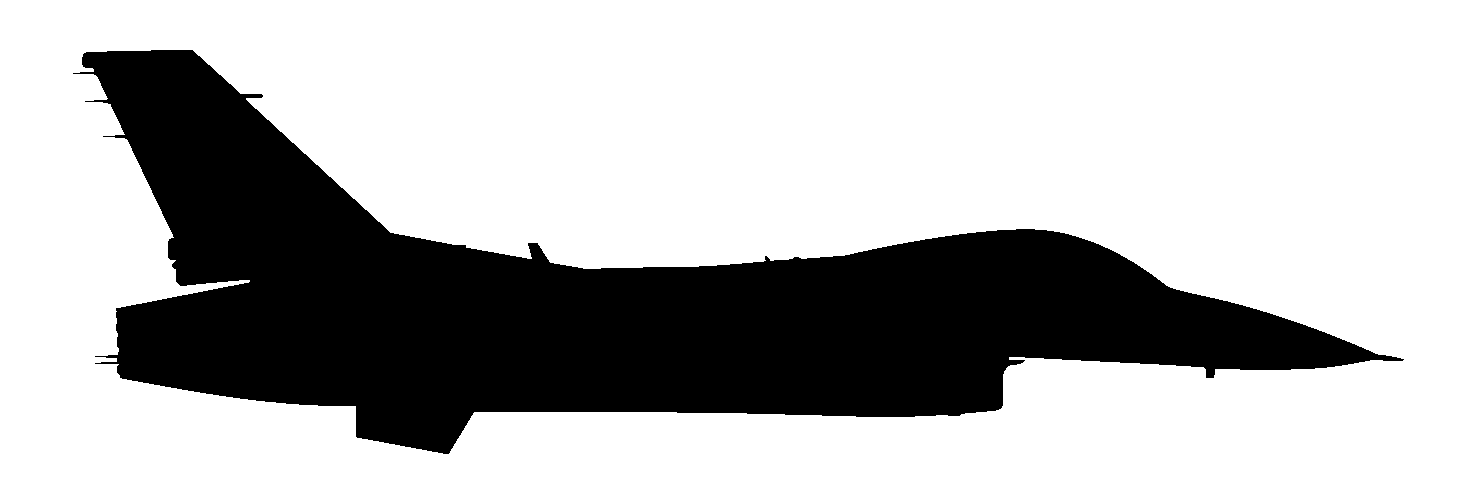
\includegraphics[
                width=7.5mm,
            ]{diagrams/aircraft/silhouette_f16_side.pdf}
        };

        \draw[ultra thick, ->] 
        (A_fighter) -- 
        (C_fighter) .. controls ($(C_fighter)+(5,0)$) and ($(C_fighter)+(5,-5)$) .. 
        ($(C_fighter)+(0,-5)$) --
        (D_fighter);

        \node[above right] at (C_fighter) {\titlefont C};
        \node[left] at (D_fighter) {\titlefont D};

        % BANDIT
        \coordinate (A_bandit) at (100,0);
        \coordinate (C_bandit) at (85,0);
        \coordinate (D_bandit) at (D_missile);

        \draw[ultra thick, ->] 
        (A_bandit) -- 
        (D_bandit);

        \node[above] at (A_bandit) {\titlefont A};
        \node[above] at (C_bandit) {\titlefont C};

        \filldraw[red] (D_bandit) circle (2pt);

        % Distance lines
        \draw[thin, <->]
        ($(C_fighter)+(0,-12.5)$) -- node[pos=0.5, above]{\small\titlefont R\textsubscript{A-POLE}}
        ($(C_bandit)+(0,-12.5)$);
        \draw[thin, <->]
        (15,-20) -- node[pos=0.5, above]{\small\titlefont R\textsubscript{F-POLE}}
        ($(D_missile)+(0,-20)$);
        \draw[thin, <->]
        ($(A_missile)+(0,-27.5)$) -- node[pos=0.5, above]{\small\titlefont R\textsubscript{LAUNCH}}
        ($(A_bandit)+(0,-27.5)$);

        \draw[thin]
        ($(C_fighter)+(0,-2.5)$) -- ($(C_fighter)+(0,-15)$)
        ($(C_bandit)+(0,-2.5)$) -- ($(C_bandit)+(0,-15)$)
        ($(D_fighter)+(0,-2.5)$) -- (15,-22.5)
        ($(D_missile)+(0,-2.5)$) -- ($(D_missile)+(0,-22.5)$)
        ($(A_missile)+(0,-2.5)$) -- ($(A_missile)+(0,-30)$)
        ($(A_bandit)+(0,-2.5)$) -- ($(A_bandit)+(0,-30)$);

    \end{tikzpicture}
    \caption{Side-on view of a generic AIM-120 employment profile}
    \label{fig:aa_weap:bvr:aim120profile}
    % TODO: silhouettes?
\end{figure}

\begin{tcoloritemize}
    \blueitem[AIM-120 \break Employment \break Profile]
    \Cref{fig:aa_weap:bvr:aim120profile} shows the trajectories of fighter, bandit \& missile for a generic AIM-120 employment profile
    including the following phases

    \begin{itemize}
        \item \textbf{A --- Launch / Boost Phase}
        \item \textbf{B --- Mid-Course Phase}
        \item \textbf{C --- Acquisition}
        \item \textbf{D --- Intercept}
    \end{itemize}
    \blueitem[Launch / Boost Phase]
    \textbf{Boost}

    \begin{itemize}
        \item Motor only fires for initial seconds of flight 
        \item After burnout missile \textbf{\underline{cannot gain energy}}
    \end{itemize}

    \textbf{Lofting} 

    \begin{itemize}
        \item To reach longer ranges missile ``lofts'' itself to conserve energy \& optimize trajectory
        \item Pilot can manually loft by raising the nose 20-30 deg prior to launch
    \end{itemize}
    \blueitem[Mid-Course Phase]
    \textbf{Missile flies using internal IMU}

    \begin{itemize}
        \item Receives periodic datalink updates
        \item Will fly to last updated target position if DL lost
    \end{itemize}
    \blueitem[Acquisition \& MPRF ``Active'' Phase]
    \textbf{Missile radar turns on once close to target location}
    \begin{itemize}
        \item Seeker in MPRF (Medium Pulse Repetition Frequency) mode 
        \item Locks on to closest / best target
    \end{itemize}
    \blueitem[Terminal Phase \& Intercept]
    \textbf{Once missile seeker has acquired target}
    \begin{itemize}
        \item Flies PNG intercept trajectory
        \item Requires no further DL support, fighter can turn away from the bandit
    \end{itemize}
\end{tcoloritemize}

\cautionbox{
    \textbf{Do NOT employ AIM-120 without clear avenue-of-fire} 
    \begin{itemize}
        \item AIM-120 has NO IFF functionality
    \end{itemize}
}

\subsubsection{TACTICAL CONSIDERATIONS}
\label{subsec:bvr:tacticalconsideration}
% \label{subsec:aim120:tactics}
\begin{tcoloritemize}
    \blueitem[Range Definitions]
    \textbf{Fighter-bandit distance} can be measured at different points during the timeline

    \begin{itemize}
        \item \textbf{R\textsubscript{Launch}} --- distance at launch
        \item \textbf{R\textsubscript{A-Pole}} --- distance when missile goes active
        \item \textbf{R\textsubscript{F-Pole}} --- distance at impact
    \end{itemize}
    
    These are also illustrated in \cref{fig:aa_weap:bvr:aim120profile}.
    \blueitem[Maximizing Launch Range / Energy]
    \textbf{Why?}
    \begin{itemize}
        \item Ability to launch at longer ranges forces bandit defensive
        \item Bandit may not be able to counter-launch
        \item Higher launch energy increases P\textsubscript{intercept} %probability of intercept
    \end{itemize}
    \textbf{How?}
    \begin{itemize}
        \item \textbf{High velocity} --- increases kinetic energy 
        \item \textbf{High altitude} --- increases potential energy, reduces drag
    \end{itemize}
    \blueitem[Maximizing \break F-Pole Range]
    \textbf{Why?}
    \begin{itemize}
        \item Less likely to enter bandit launch envelope
        \item More time/range to launch 2nd missile if necessary
    \end{itemize}
    \textbf{How?}
    \begin{itemize}
        \item \textbf{Crank} --- turn 45-60 degrees away from bandit to reduce closure rate, maintain radar contact
        \item \textbf{Dive} --- reduces threat missile envelope
    \end{itemize}
    \blueitem[Flowing Cold]
    \textbf{Why?}
    \begin{itemize}
        \item Missile requires no support once active
        \item Defend against unknown missile launches
        \item Maximize F-pole range further
    \end{itemize}
    \textbf{How?}
    \begin{itemize}
        \item \textbf{Turn} --- Away from bandit / threat
        \item \textbf{Dive} --- if necessary, reduces threat missile envelope 
    \end{itemize}
    \blueitem[Effect of Bandit Maneuvers]
    As evident in \cref{fig:aa_weap:bvr:aim120profile}, 
   \textbf{R\textsubscript{Launch}} is significantly greater than the distance travelled by the missile
    \begin{itemize}
        \item \textbf{DLZ calculated based off \underline{both} fighter \underline{and} bandit velocity/altitude}
        \item Bandit can significantly change missile envelope by reducing closure rate / altitude
        \item Post-launch bandit maneuvers can result in missile not having energy to intercept
    \end{itemize}
\end{tcoloritemize}

\clearpage

\subsection{FIGHTER MANEUVERS}

\begin{tcoloritemize}
    \blueitem[Crank]
    Fighter turns \textbf{45-60 deg} away from threat 

    \begin{itemize}
        \item reduces closure while maintaining radar track
        \item typically used post-launch
    \end{itemize}
    
    Reference \cref{fig:aa_weap:bvr:fightermaneuver:crank}
    \blueitem[Notch]
    Fighter turns \textbf{70-110 deg} away from threat

    \begin{itemize}
        \item minimizes relative velocity to break hostile pulse-doppler radar track
        \item increases angular motion, forcing missile to maneuver and expend energy
    \end{itemize}
    
    Reference \cref{fig:aa_weap:bvr:fightermaneuver:notch}
    \blueitem[Go Cold]
    Fighter turns \textbf{away} from threat

    \begin{itemize}
        \item used to kinematically defeat threat missiles
    \end{itemize}
    
    Reference \cref{fig:aa_weap:bvr:fightermaneuver:cold}
\end{tcoloritemize}

\begin{figure}[htbp]
    \centering
    \begin{subfigure}[b]{0.3\linewidth}
        \centering
        \begin{tikzpicture}[figstyle]
            % FIGHTER
            \node[
                anchor=north,
                yshift=1mm,
            ] (fighter) at (0,0) {
                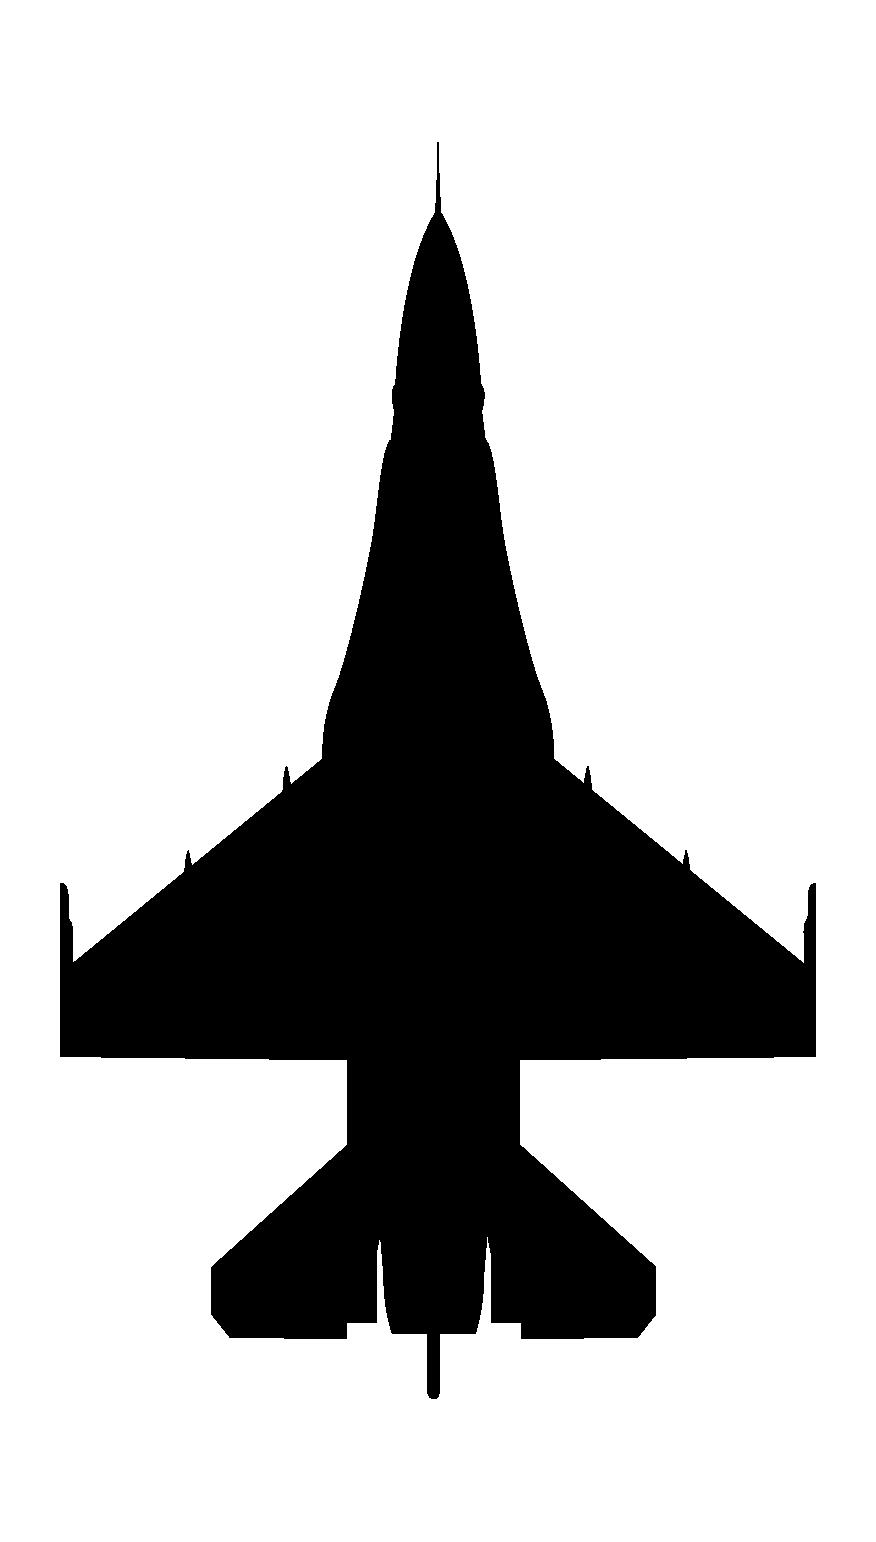
\includegraphics[
                    width=7.5mm,
                ]{diagrams/aircraft/silhouette_f16_top.pdf}
            };
            \draw[rounded corners, ->] 
            (0,0) -- (0,5) -- +(30:15) node[rotate=-60, anchor=south, yshift=-1mm]{
                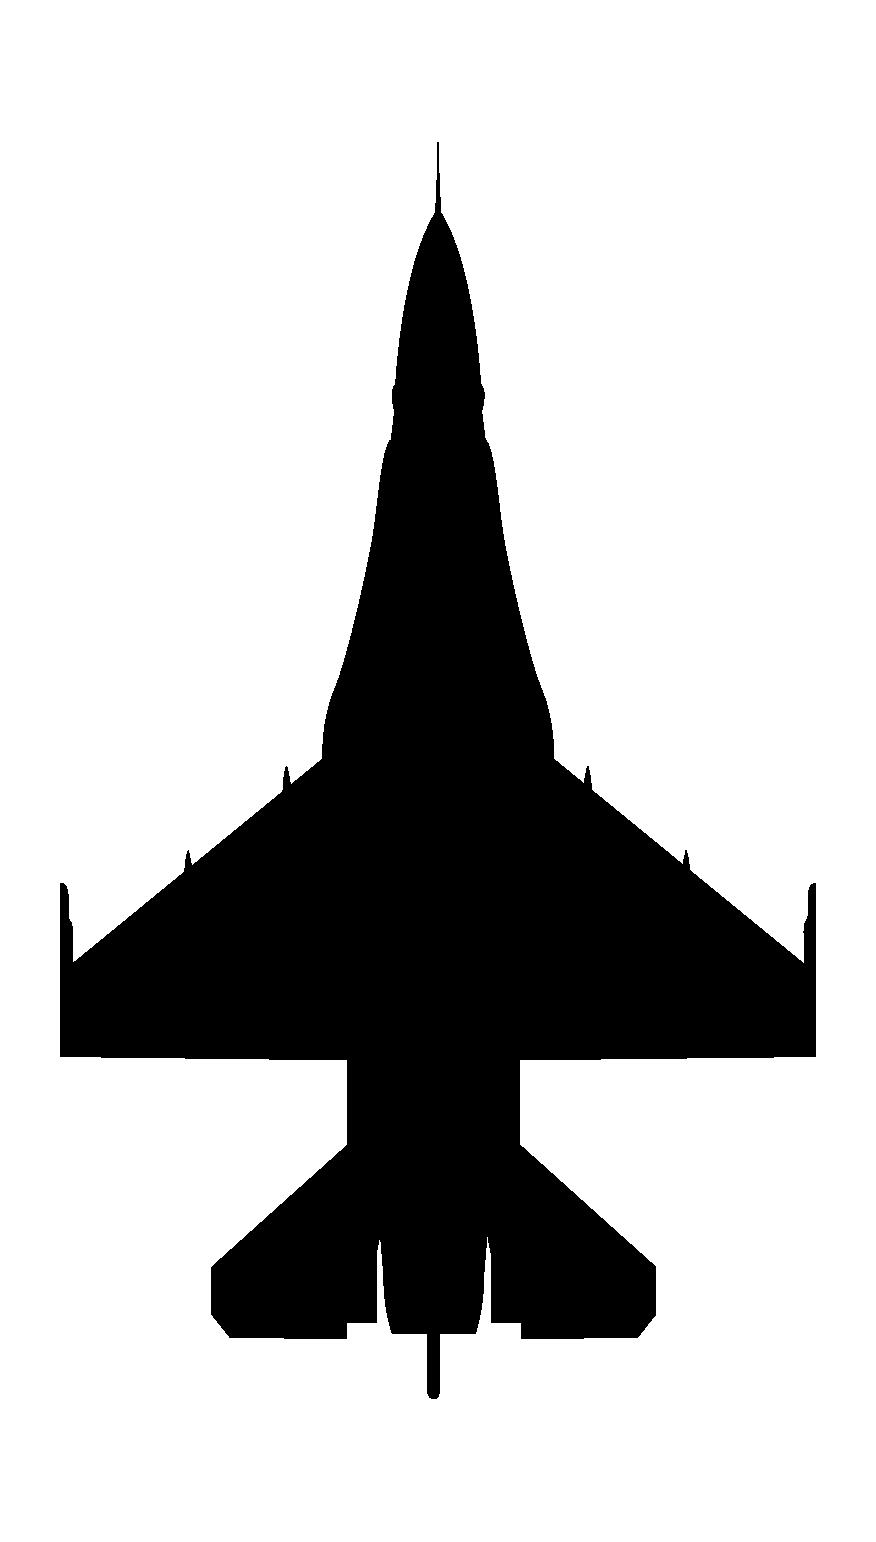
\includegraphics[
                width=7.5mm,
            ]{diagrams/aircraft/silhouette_f16_top.pdf}};
    
            % BANDIT
            \draw[rounded corners, ->] 
            (0,35) -- (0,25);
    
            % help line
            \draw[thin, dashed] 
            (0,25) -- (0,5);
    
            \draw[thin]
            (0,15) arc (90:30:10) node[pos=0.15, above right]{\small\titlefont 45-60$^\circ$};
    
        \end{tikzpicture}
        \caption{Crank}
        \label{fig:aa_weap:bvr:fightermaneuver:crank}
    \end{subfigure}
    \begin{subfigure}[b]{0.3\linewidth}
        \centering
        \begin{tikzpicture}[figstyle]
            % FIGHTER
            \node[
                anchor=north,
                yshift=1mm,
            ] (fighter) at (0,0) {
                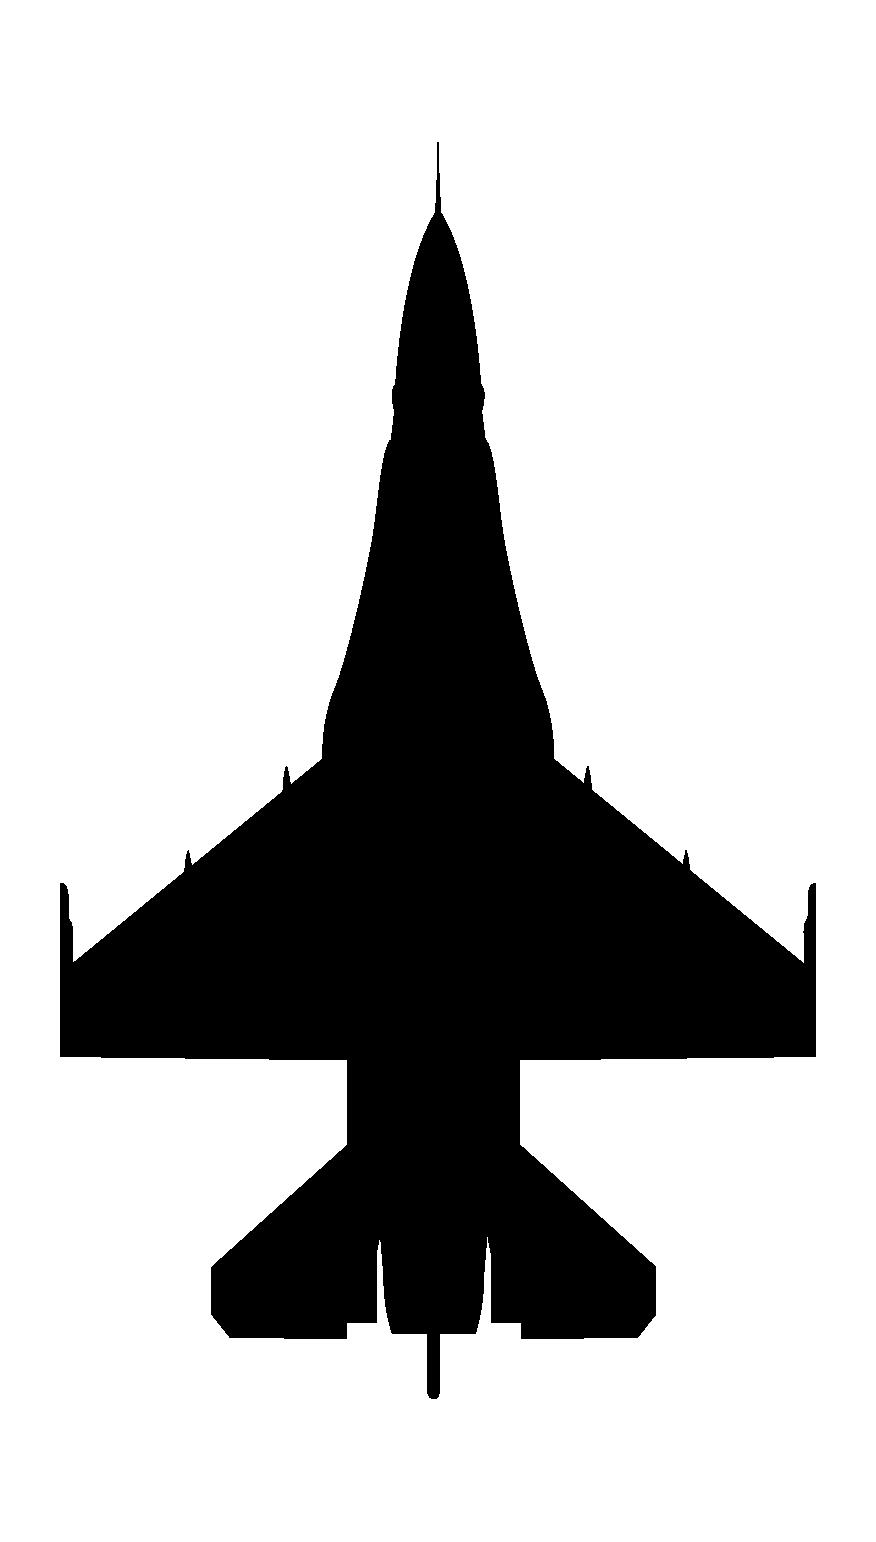
\includegraphics[
                    width=7.5mm,
                ]{diagrams/aircraft/silhouette_f16_top.pdf}
            };
            \draw[rounded corners, ->] 
            (0,0) -- (0,5) -- +(0:15) node[rotate=-90, anchor=south, yshift=-1mm]{
                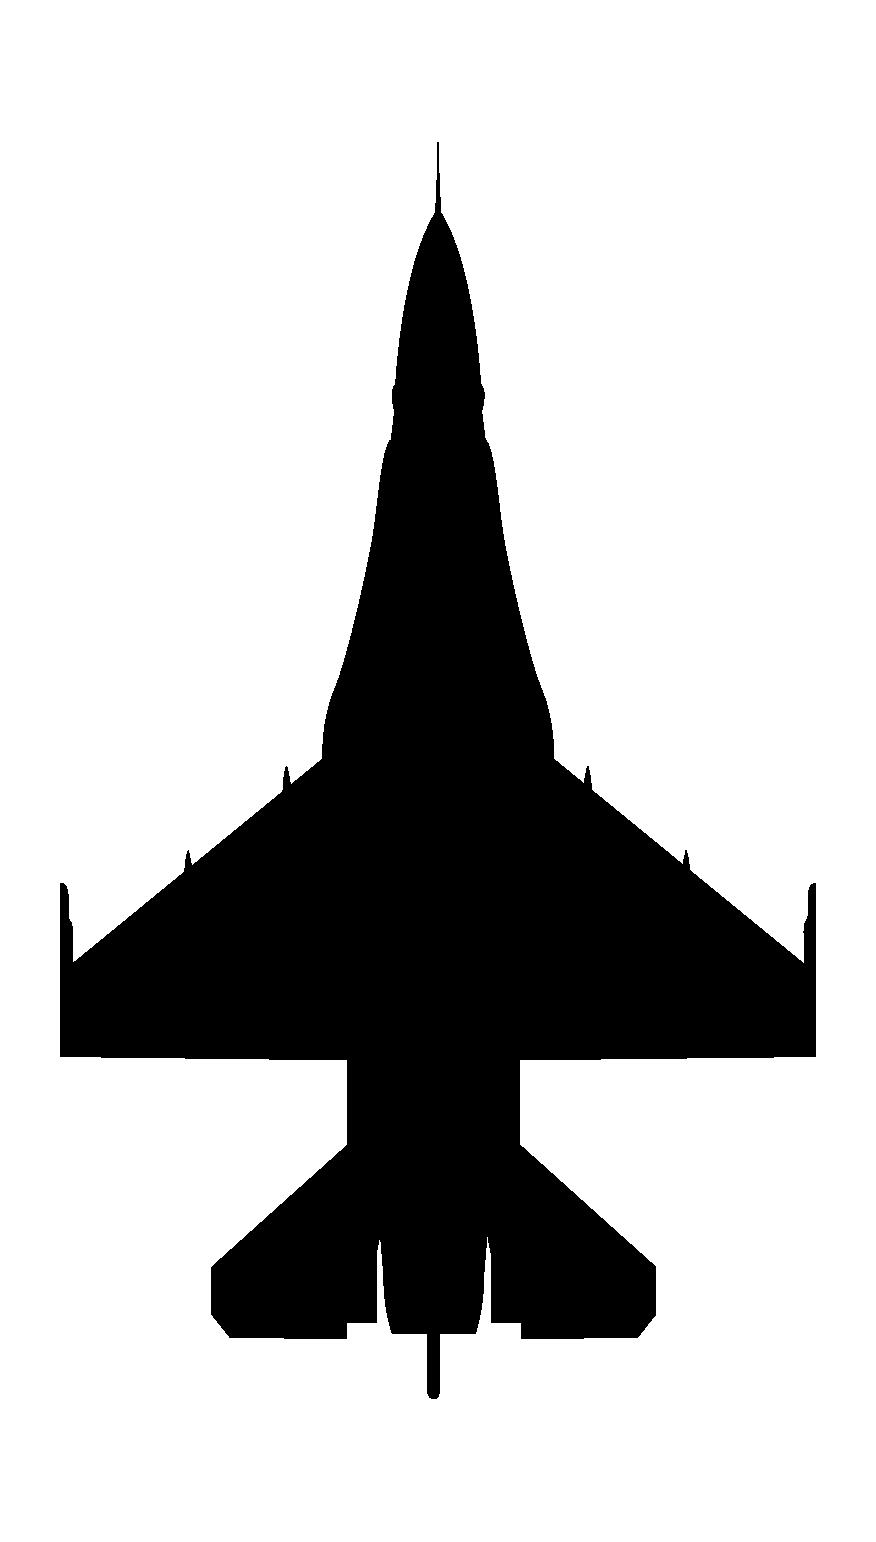
\includegraphics[
                width=7.5mm,
            ]{diagrams/aircraft/silhouette_f16_top.pdf}};
    
            % BANDIT
            \draw[rounded corners, ->] 
            (0,35) -- (0,25);
    
            % help line
            \draw[thin, dashed] 
            (0,25) -- (0,5);
    
            \draw[thin]
            (0,15) arc (90:0:10) node[pos=0.5, above right]{\small\titlefont 70-110$^\circ$};
    
        \end{tikzpicture}
        \caption{Notch}
        \label{fig:aa_weap:bvr:fightermaneuver:notch}
    \end{subfigure}
    \begin{subfigure}[b]{0.3\linewidth}
        \centering
        \begin{tikzpicture}[figstyle]
            % FIGHTER
            \node[
                anchor=north,
                yshift=1mm,
            ] (fighter) at (0,0) {
                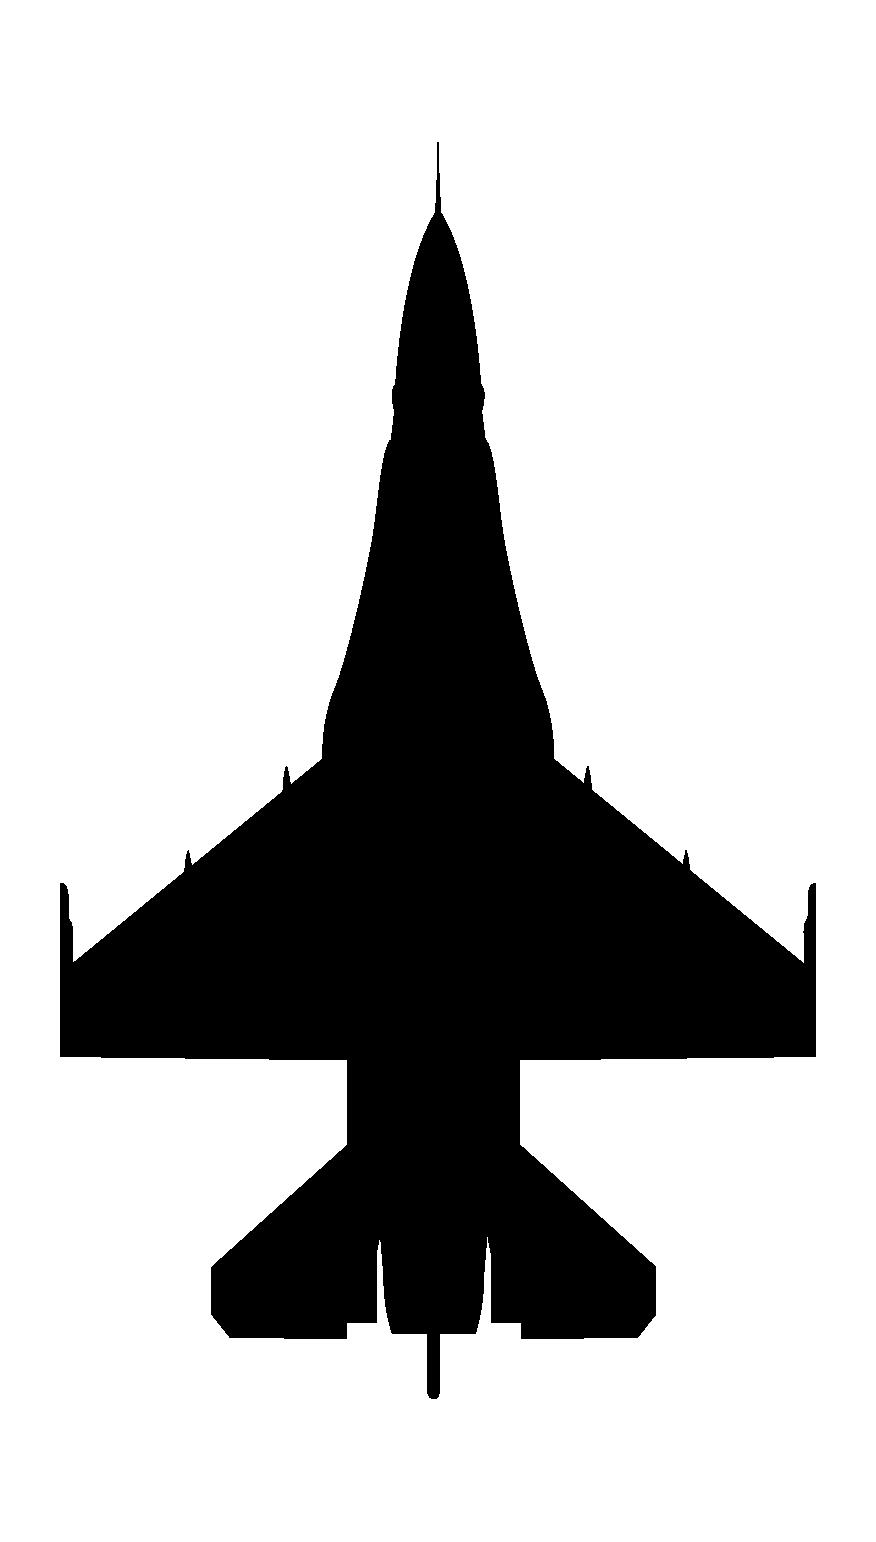
\includegraphics[
                    width=7.5mm,
                ]{diagrams/aircraft/silhouette_f16_top.pdf}
            };
            \draw[->] 
            (0,0) -- 
            (0,5) arc (180:0:5) --
            (10,0) 
            node[rotate=-180, anchor=south, yshift=-1mm]{
                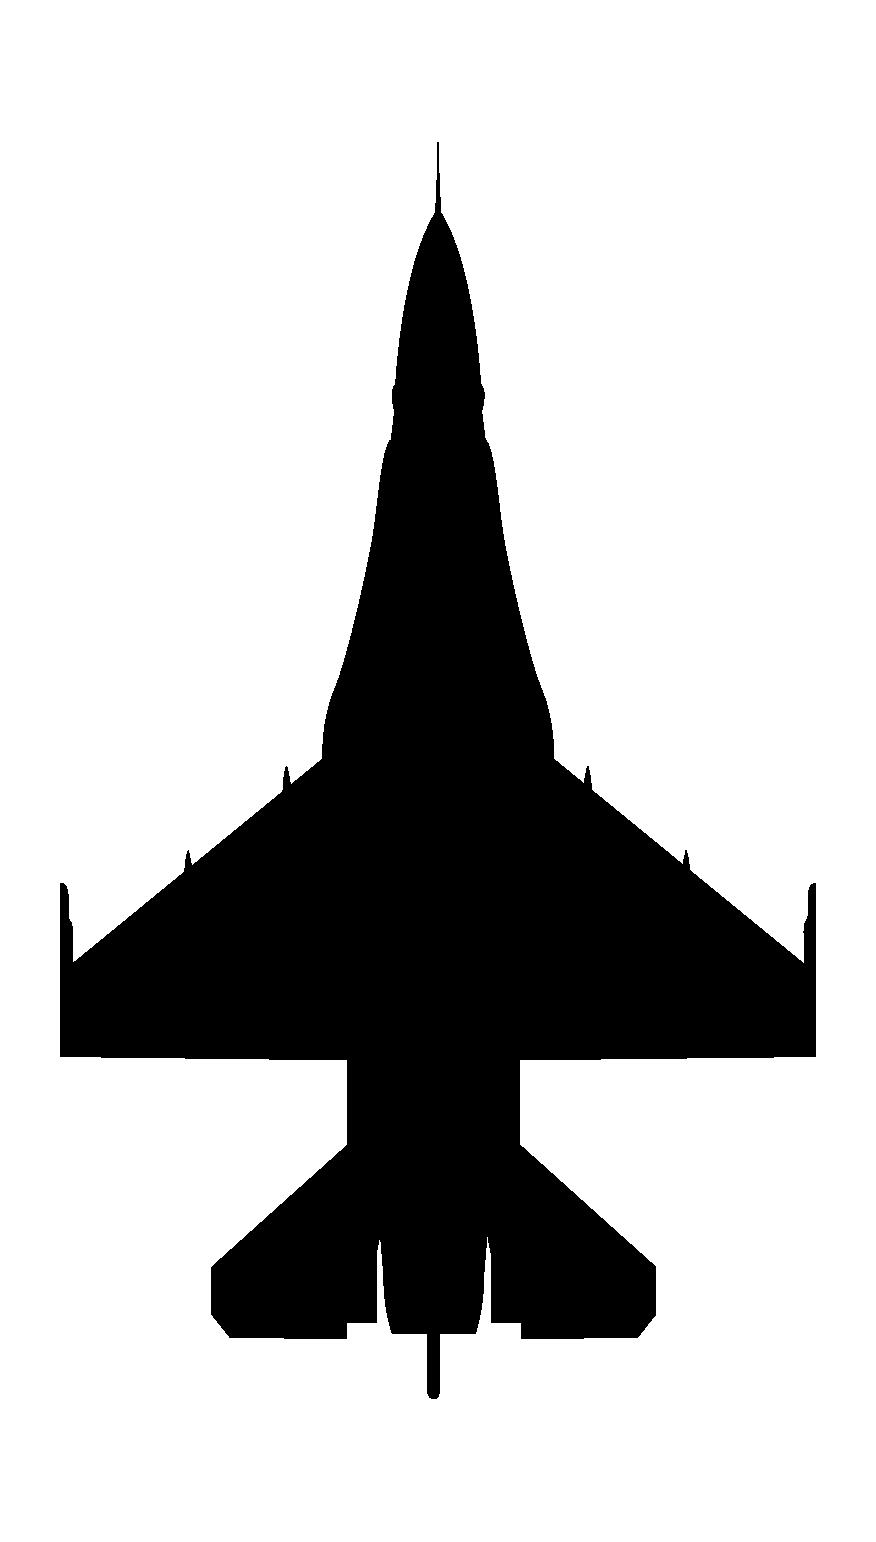
\includegraphics[
                width=7.5mm,
            ]{diagrams/aircraft/silhouette_f16_top.pdf}};
    
            % BANDIT
            \draw[rounded corners, ->] 
            (0,35) -- (0,25);

            % help line
            \draw[thin, dashed] 
            (0,25) -- (0,5);

        \end{tikzpicture}
        \caption{Go Cold}
        \label{fig:aa_weap:bvr:fightermaneuver:cold}
    \end{subfigure}
    \caption{Top-down view of basic BVR fighter maneuvers}
    \label{fig:aa_weap:bvr:fightermaneuver}
\end{figure}

\notebox{
    \textbf{Turning in after going cold can place fighter within bandit launch envelope}
}

\subsection{TARGET ASPECT}

\begin{tcoloritemize}
    \blueitem[Target Aspect]
    Angle between imaginary line connecting fighter-bandit and bandit heading
    \blueitem[Hot]
    \textbf{Target aspect --- 0-40 deg}
    \begin{itemize}
        \item offensive posture, maximizes closure
    \end{itemize}
    \blueitem[Flank]
    \textbf{Target aspect --- 40-70 deg}
    \begin{itemize}
        \item minimizes closure while maintaining radar track
    \end{itemize}
    \blueitem[Beam]
    \textbf{Target aspect --- 70-110 deg}
    \begin{itemize}
        \item defensive maneuver to break pulse-doppler radar track
    \end{itemize}
    \blueitem[Drag]
    \textbf{Target aspect --- 110-180 deg}
    \begin{itemize}
        \item defense to kinematically defeat missile
        \item often used in group tactics as ambush setup
    \end{itemize}
\end{tcoloritemize}

\begin{figure}[htbp]
    \centering
    \begin{subfigure}[b]{0.2\linewidth}
        \centering
        \begin{tikzpicture}[figstyle]
            % FIGHTER
            \node[
                anchor=north,
                yshift=1mm,
            ] (fighter) at (0,0) {
                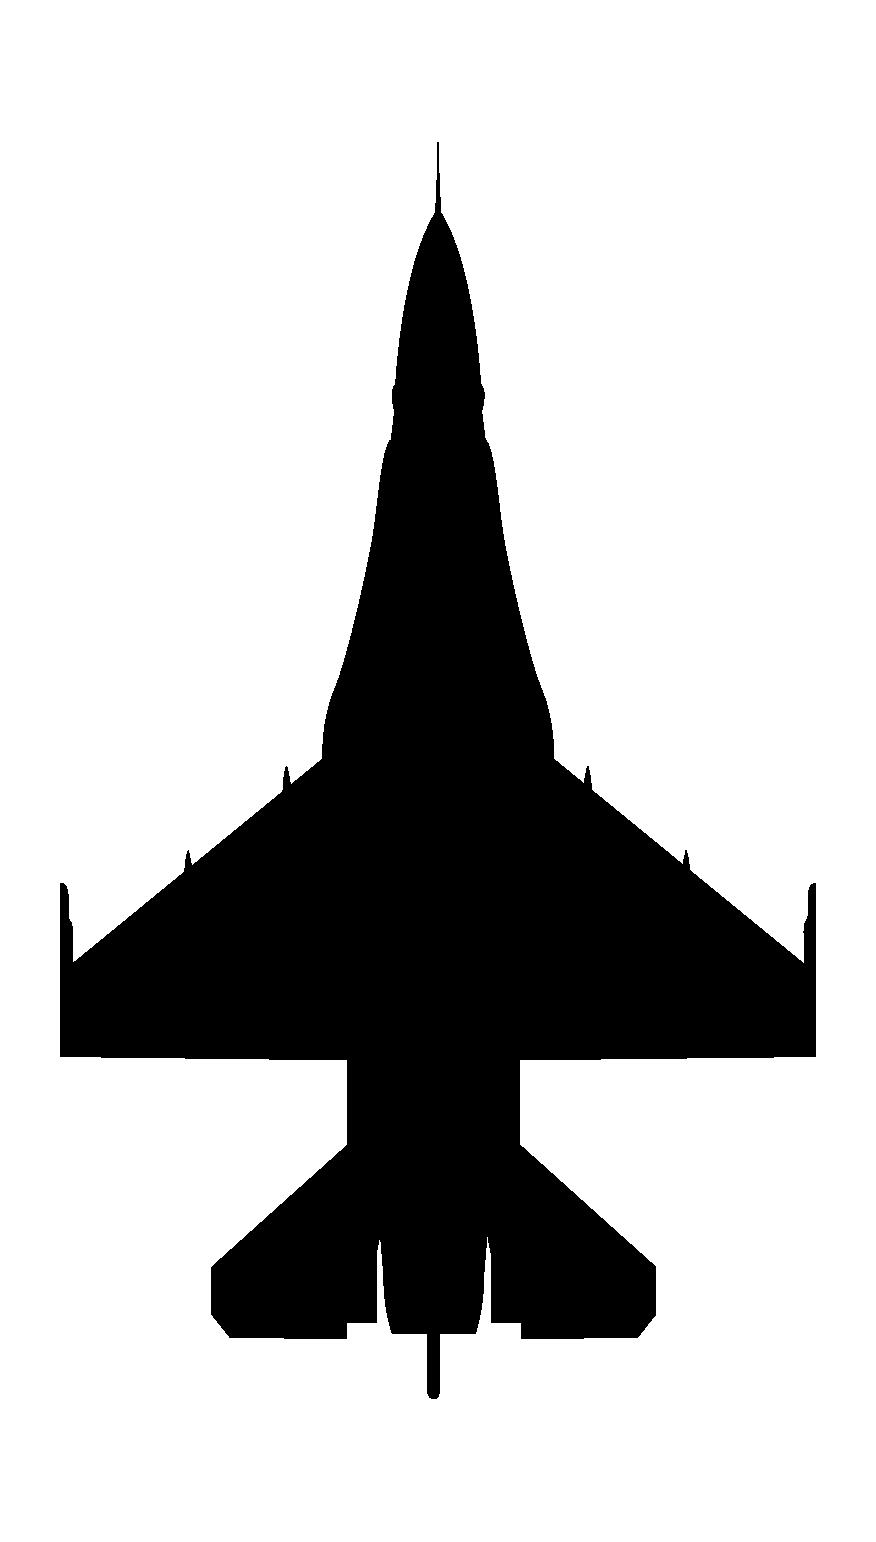
\includegraphics[
                    width=7.5mm,
                ]{diagrams/aircraft/silhouette_f16_top.pdf}
            };
    
            % BANDIT
            \draw[rounded corners, ->] 
            (0,20) -- +(-75:15);
    
            % help line
            \draw[thin, dashed] 
            (0,20) -- (0,0);
    
            \draw[thin]
            (0,10) arc (-90:-75:10) node[pos=1.0, right]{\small\titlefont 0-40$^\circ$};

        \end{tikzpicture}
        \caption{Hot}
        \label{fig:aa_weap:bvr:ta:hot}
    \end{subfigure}
    \begin{subfigure}[b]{0.2\linewidth}
        \centering
        \begin{tikzpicture}[figstyle]
            % FIGHTER
            \node[
                anchor=north,
                yshift=1mm,
            ] (fighter) at (0,0) {
                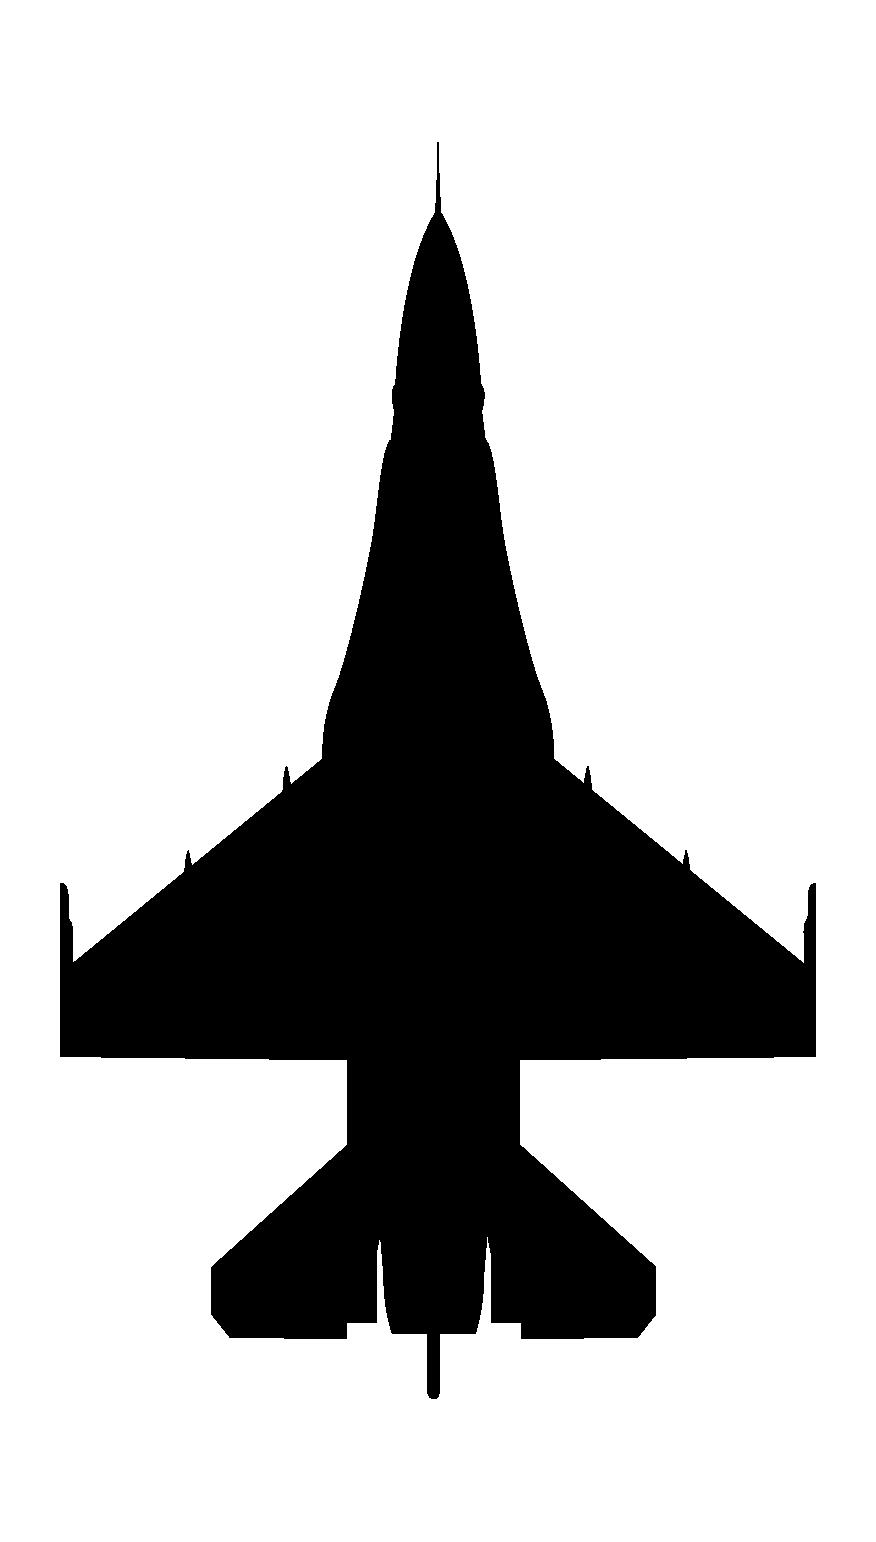
\includegraphics[
                    width=7.5mm,
                ]{diagrams/aircraft/silhouette_f16_top.pdf}
            };
    
            % BANDIT
            \draw[rounded corners, ->] 
            (0,20) -- +(-30:15);
    
            % help line
            \draw[thin, dashed] 
            (0,20) -- (0,0);
    
            \draw[thin]
            (0,10) arc (-90:-30:10) node[pos=0.25, below right]{\small\titlefont 40-70$^\circ$};

        \end{tikzpicture}
        \caption{Flank}
        \label{fig:aa_weap:bvr:ta:flank}
    \end{subfigure}
    \begin{subfigure}[b]{0.25\linewidth}
        \centering
        \begin{tikzpicture}[figstyle]
            % FIGHTER
            \node[
                anchor=north,
                yshift=1mm,
            ] (fighter) at (0,0) {
                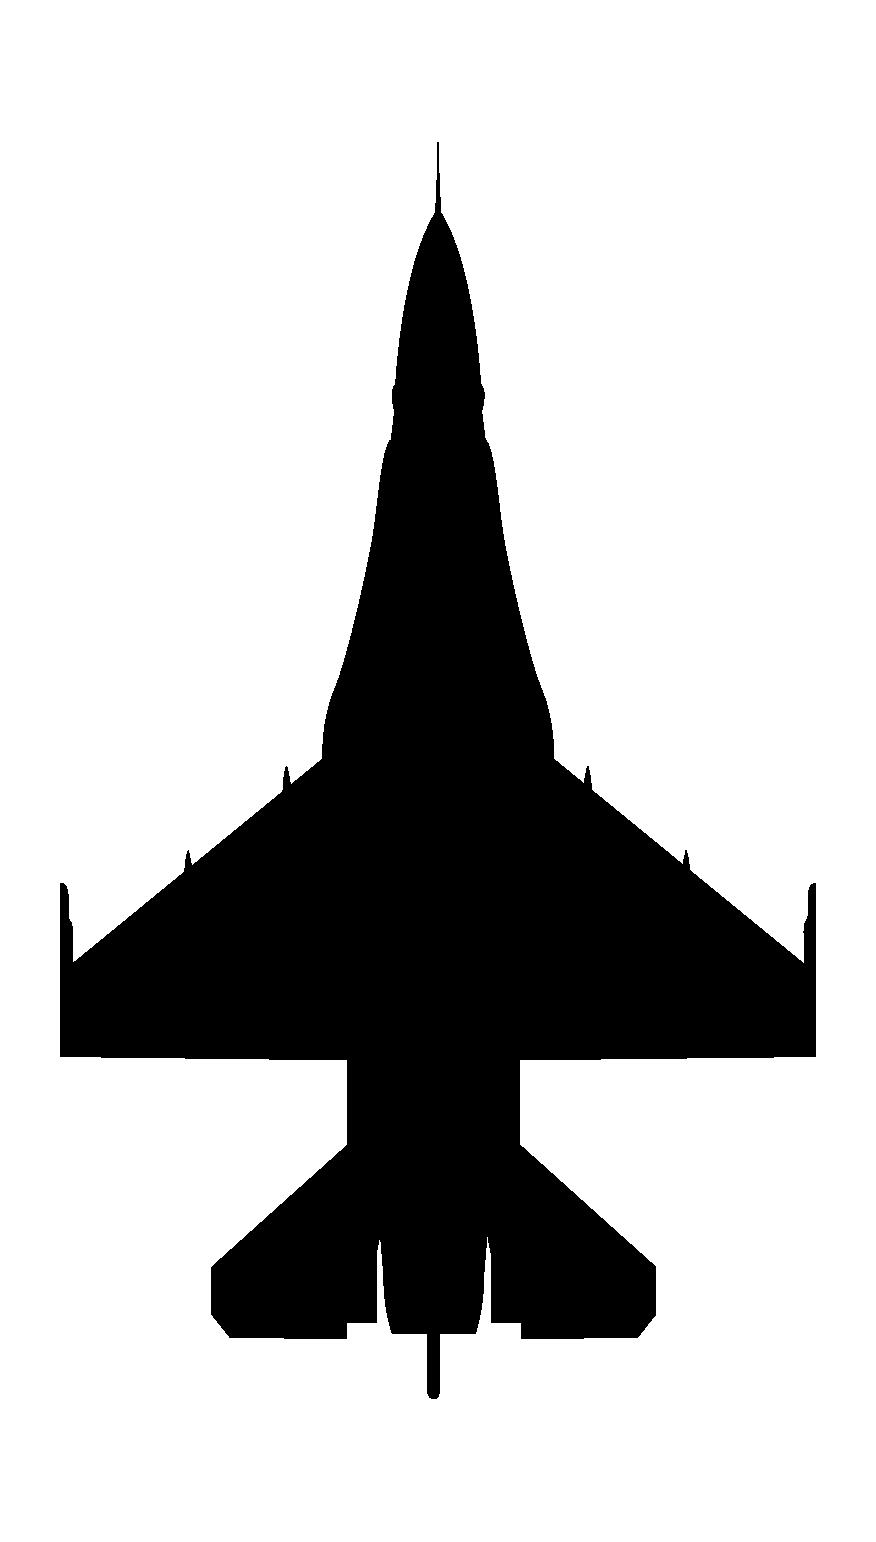
\includegraphics[
                    width=7.5mm,
                ]{diagrams/aircraft/silhouette_f16_top.pdf}
            };
    
            % BANDIT
            \draw[rounded corners, ->] 
            (0,20) -- +(0:15);
    
            % help line
            \draw[thin, dashed] 
            (0,20) -- (0,0);
    
            \draw[thin]
            (0,10) arc (-90:0:10) node[pos=0.25, below right]{\small\titlefont 70-110$^\circ$};
    
        \end{tikzpicture}
        \caption{Beam}
        \label{fig:aa_weap:bvr:ta:beam}
    \end{subfigure}
    \begin{subfigure}[b]{0.25\linewidth}
        \centering
        \begin{tikzpicture}[figstyle]
            % FIGHTER
            \node[
                anchor=north,
                yshift=1mm,
            ] (fighter) at (0,0) {
                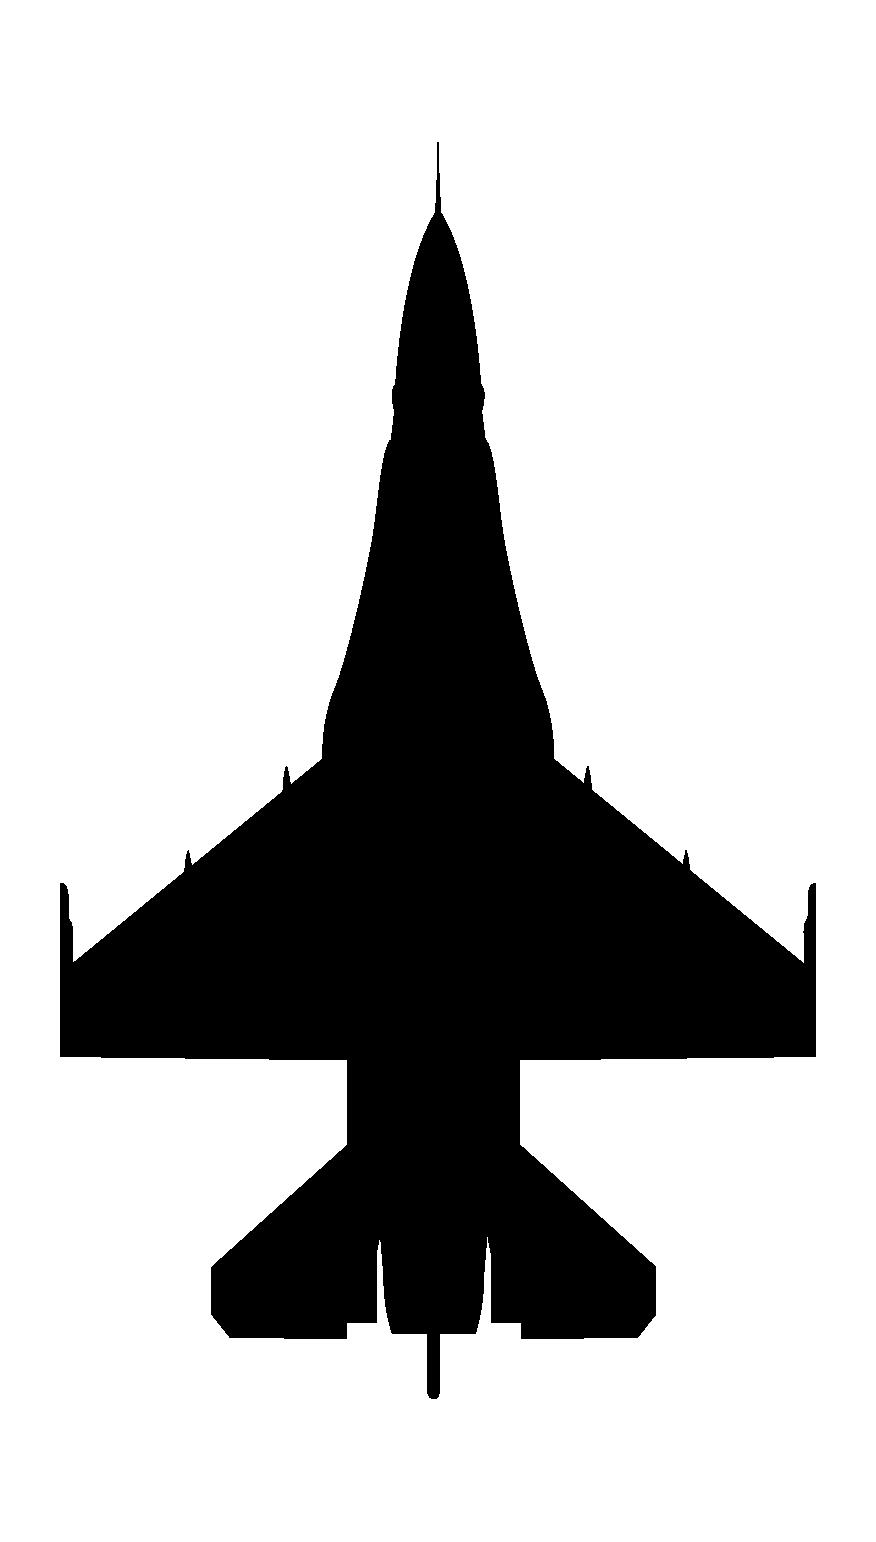
\includegraphics[
                    width=7.5mm,
                ]{diagrams/aircraft/silhouette_f16_top.pdf}
            };
    
            % BANDIT
            \draw[rounded corners, ->] 
            (0,20) -- +(90:15);
    
            % help line
            \draw[thin, dashed] 
            (0,20) -- (0,0);
    
            \draw[thin]
            (0,10) arc (-90:90:10) node[pos=0.125, below right]{\small\titlefont 110-180$^\circ$};
    
        \end{tikzpicture}
        \caption{Drag}
        \label{fig:aa_weap:bvr:ta:drag}
    \end{subfigure}
    \caption{Top down view illustrating target aspect classification}
    \label{fig:aa_weap:bvr:ta}
\end{figure}

\clearpage
\section{INTERCEPT TIMELINES}

\subsection{TERMINOLOGY}

\begin{tcoloritemize}
    \blueitem[Contact]
    \blueitem[Group]
    \blueitem[Picture]
\end{tcoloritemize}

\subsection[AR FLOW]{ACTIVE-RADAR MISSILE FLOW}

\begin{tcoloritemize}
    \blueitem[Launch-and-Leave]
    Launch-and-leave tactics utilize AIM-120 terminal guidance independence 
    to defeat bandit missiles though out maneuvers, 
    with the fighter turning cold once AIM-120 has gone active.

    \bigskip
    \textbf{Skate} \hfill see \cref{subsec:ttpaa:timeline:skate}\\
    AIM-120 launched before a briefed tranisition range 
    such that it goes active before fighters reach a desired out range.
    Fighters go out before recommitting for a second launch.
    
    \bigskip
    \textbf{Short-Skate} \hfill see \cref{subsec:ttpaa:timeline:shortskate}\\
    AIM-120 launched such that fighter can go out before reaching MAR.

    \blueitem[Launch-and-Decide]
    Launch-and-decide tactics also utilize AIM-120 terminal guidance independence, 
    allowing fighter to decide whether to abort out or continue in.

    \bigskip
    \textbf{Banzai} \hfill see \cref{subsec:ttpaa:timeline:banzai}\\
    Fighter launches before a briefed decision range and goes into notch for predetermined duration. 
    Can abort out or continue in depending on if spiked/naked and bandit maneuver.

    Typically employed with elements cranking in opposite directions, increasing chance of 1 fighter being naked
\end{tcoloritemize}


\subsection{RANGE DEFINITIONS}

\begin{tcoloritemize}
    \blueitem[Bandit WEZ] \textbf{W}eapon \textbf{E}ngagement \textbf{Zone}

    \medskip
    range at which bandit weapons can engage fighter, synonomous with bandit R\textsubscript{F-pole} in this document

    \blueitem[MAR] \textbf{M}inimum \textbf{A}bort \textbf{R}ange

    \medskip
    minimum range at which fighter can perform an abort maneuver to kinematically defeat any launched bandit weapons 

    \medskip
    \textbf{MAR} = max bandit R\textsubscript{F-pole} + fighter turn radius
    \blueitem[MSR] \textbf{M}inimum \textbf{S}hot \textbf{R}ange

    \medskip
    minimum range at which AIM-120 will go active before fighter reaches MAR if launched

    \blueitem[DOR] \textbf{D}esired \textbf{O}ut \textbf{R}ange

    \medskip
    minimum range at which fighter can go out, defeating bandit missiles, 
    before recommitting to a second employment with launch-and-decide tactics

    \blueitem[TR] \textbf{T}ransition \textbf{R}ange

    \medskip
    minimum range at which AIM-120 will go active before fighter reaches DOR if launched
    \blueitem[MTR] \textbf{M}inimum \textbf{T}argeting \textbf{R}ange

    \medskip
    minimum range for flight to begin targeting and execute launch-and-leave tactics
    \blueitem[MRR] \textbf{M}inimum \textbf{R}ecommit \textbf{R}ange

    \medskip
    minimum range at which a fighter which is out can recommit, 
    retarget and employ an AIM-120 before going out again at MAR

    \blueitem[DR] \textbf{D}ecision \textbf{R}ange

    \medskip
    minimum range at which fighter can execute briefed notch maneuver for launch-and-decide tactics

    \medskip

    \textbf{DR} = max bandit R\textsubscript{F-pole} + bandit closure \times \ t\textsubscript{notch}
\end{tcoloritemize}

\notebox{
    \textbf{It is important to note that:}
    \begin{itemize}
        \item The timelines described in \cref{subsec:ttpaa:timeline:banzai,subsec:ttpaa:timeline:skate,subsec:ttpaa:timeline:shortskate}
        are to help illustrate core concepts of intercept timelines, \textbf{NOT} to be followed as absolute procedures.
        \item To define a proper timeline, you must define you assumptions.
        \begin{itemize}
            \item what is the bandit doing, what speed/altitude?
            \item what is the performance of bandit missiles?
            \item what tactics will the bandit most likely employ?
        \end{itemize}
        \item Specifically, defining the bandit WEZ / R\textsubscript{f-pole}, which define the MAR, 
        relies on an accurate understanding of threat missile and aircraft performance 
        as well as tactics.
        \item The timelines visualized in \cref{fig:ttpaa:timeline:banzai,fig:ttpaa:timeline:skate,fig:ttpaa:timeline:shortskate} are not to scale, 
        any crank maneuvers are ommitted for compactness and visual clarity.
        \item Rather than getting lost in the FCR page trying to execute complex tactics, 
        ensure that the fundamentals are not getting forgotten. A typical order of priority is
        \begin{enumerate}
            \item formation
            \item sensors
            \item communications
        \end{enumerate}
        in that order.
    \end{itemize}
}

\marginfigeometry

\subsection{BANZAI TIMELINE}
\label{subsec:ttpaa:timeline:banzai}

\begin{checklistenumerate}[start=0]
    \blueitem[Pre-commit] maintain SA
    
    \begin{itemize}
        \item \textbf{Comms} --- monitor AWACS
        \item \textbf{Sensors} --- sanitize airspace
    \end{itemize}

    \blueitem[Commit]%
    \label{subsec:ttpaa:timeline:banzai:commit}
    \marginpar{
        \captionsetup{type=figure}
        \centering
        \begin{tikzpicture}[figstyle]

            % coordinates
            \coordinate (fighter_start) at (0,0);
            \coordinate (bandit) at (5,75);

            \coordinate (cr) at (0,0);
            \coordinate (mtr) at (0,10);
            \coordinate (sort) at (0,17.5);
            \coordinate (shoot) at (0,25);
            \coordinate (dr) at (0,35);
            \coordinate (fighter_banzai) at (20,55);
            \coordinate (fighter_abort) at (20,30);
            \coordinate (mar) at (5,50);
            \coordinate (wez) at (0,60);

            % range lines
            \draw[thin]
                (25,0) -- (25,75);

            \path let \p1=(bandit) in 
            node[font=\footnotesize,anchor=west] at (25,\y1) {BANDIT};
            \path let \p1=(wez) in 
            node[font=\footnotesize,anchor=west] at (25,\y1) {WEZ};
            \path let \p1=(mar) in 
            node[font=\footnotesize,anchor=west] at (25,\y1) {MAR};
            \path let \p1=(dr) in 
            node[font=\footnotesize,anchor=west] at (25,\y1) {DR};
            \path let \p1=(mtr) in 
            node[font=\footnotesize,anchor=west] at (25,\y1) {MTR};
            \path let \p1=(cr) in 
            node[font=\footnotesize,anchor=west] at (25,\y1) {CR};

            \draw[thin, dashed] let \p1=(wez) in  
                (25,\y1) -- ++(-30, 0);
            \draw[thin, dashed] let \p1=(mar) in  
                (25,\y1) -- ++(-30, 0);
            \draw[thin, dashed] let \p1=(dr) in  
                (25,\y1) -- ++(-25, 0);
            \draw[thin, dashed] let \p1=(mtr) in  
                (25,\y1) -- ++(-25, 0);
            \draw[thin, dashed] let \p1=(cr) in  
                (25,\y1) -- ++(-25, 0);

            % bandit wez
            \draw[fill=red!40]
                (bandit)
                -- ++(-60:15)
                arc (-60:-120:15)
                -- (bandit);
            
            % timeline
            \draw[->] 
                (fighter_start) -- 
                node[below, pos=0]{
                    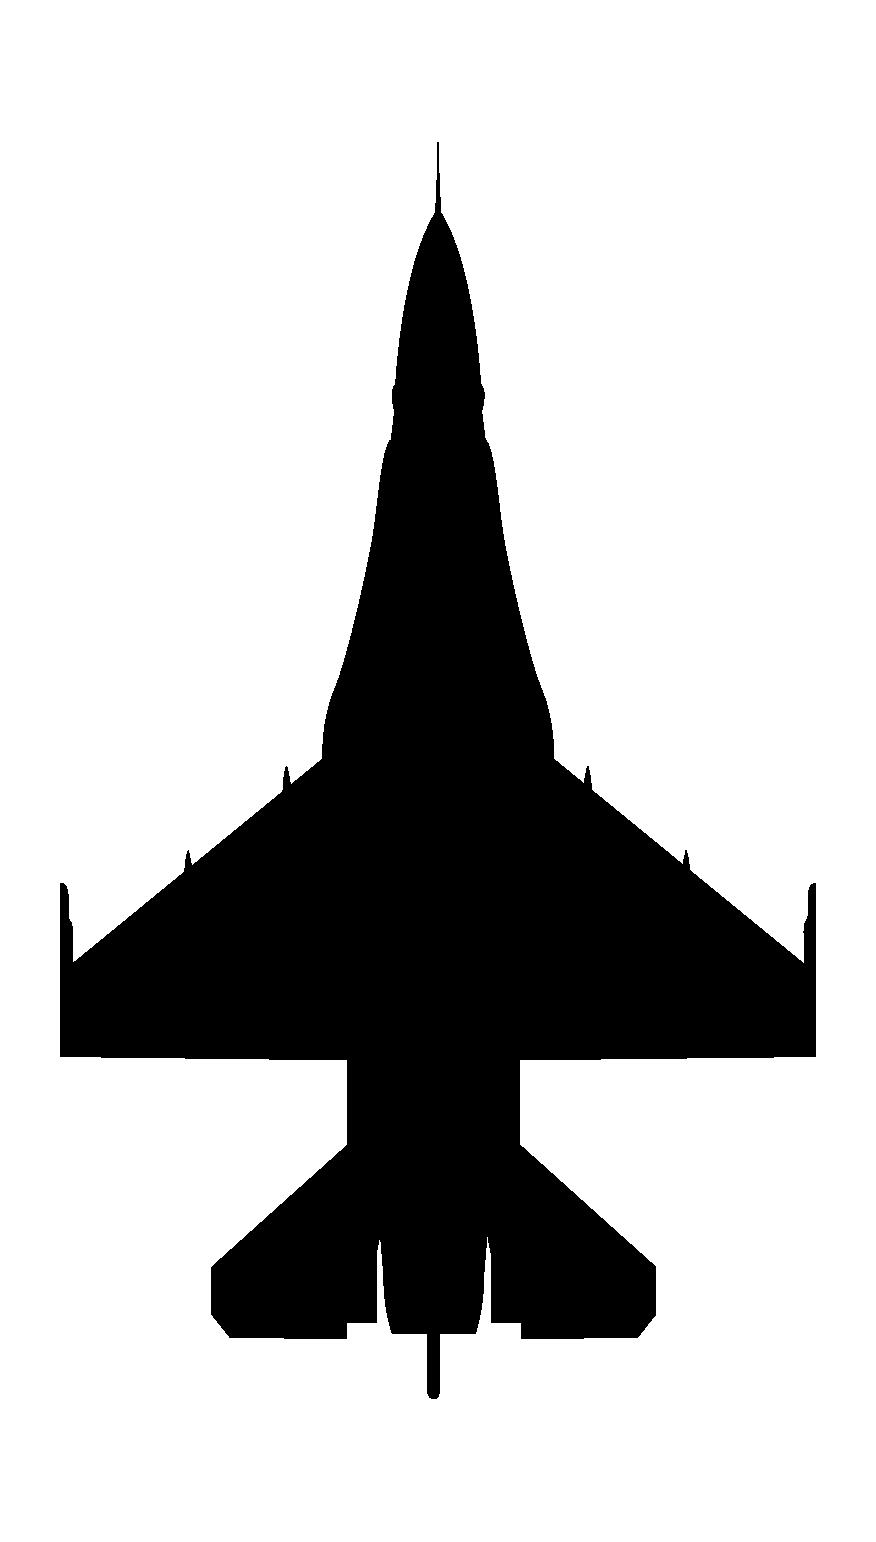
\includegraphics[
                    width=7.5mm,
                ]{diagrams/aircraft/silhouette_f16_top.pdf}} 
                (mtr);
            \draw[->]
                (mtr)
                -- (shoot);
            \draw[->]
                (shoot)
                -- (dr);
            \draw[->, dashed]
                (dr)
                arc (180:90:5) 
                -- ++(10,0)
                arc (90:0:5) 
                -- (fighter_abort)
                node[below, pos=1, ]{
                    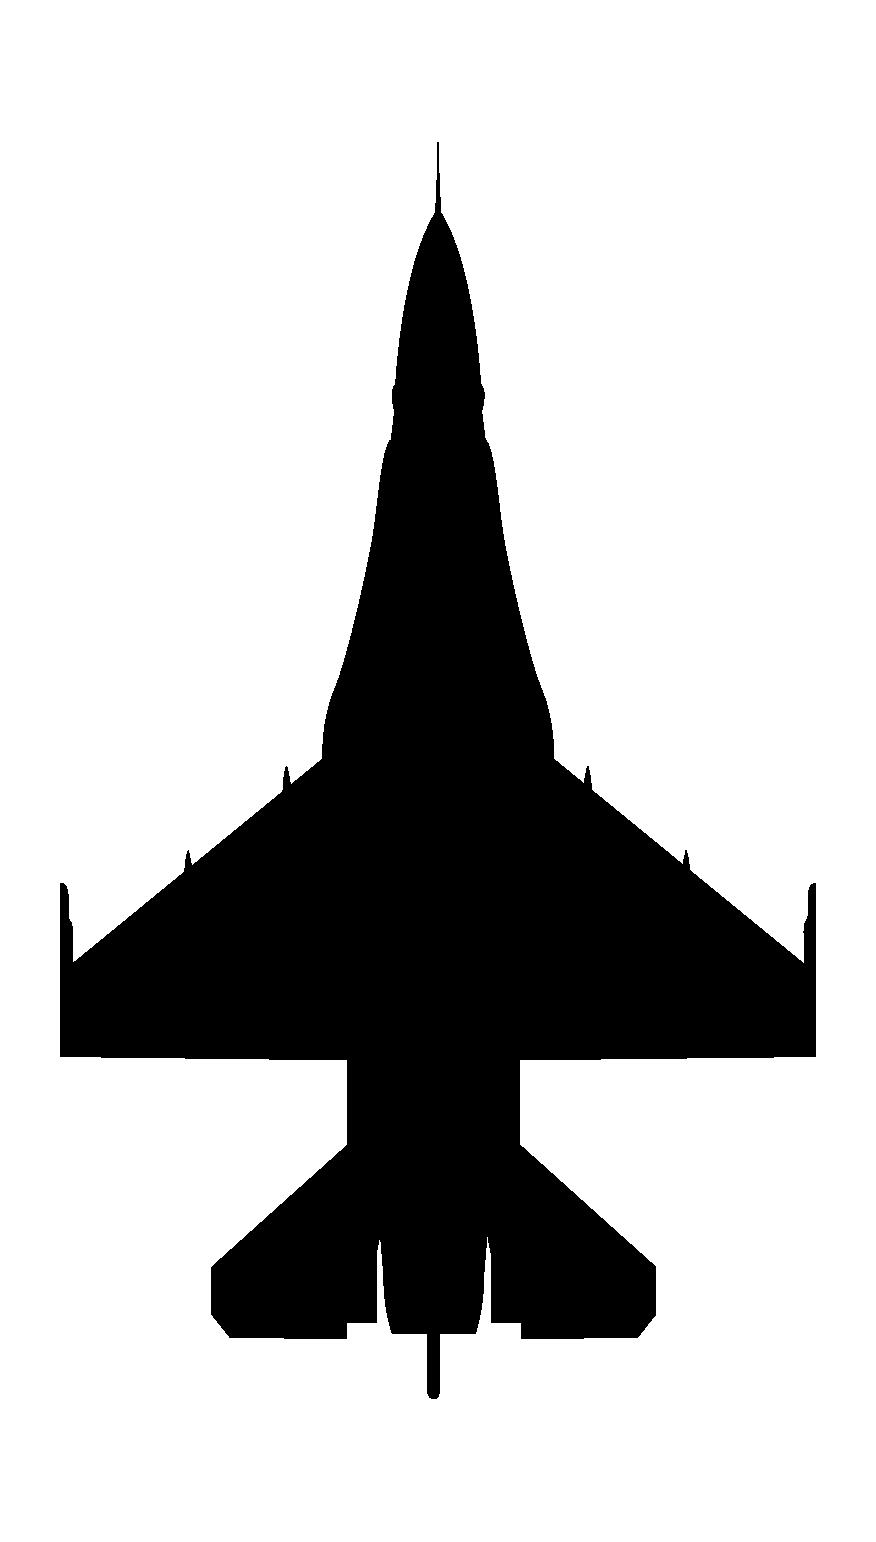
\includegraphics[
                        angle=180,
                        width=7.5mm,
                ]{diagrams/aircraft/silhouette_f16_top.pdf}};
            \draw[->]
                (dr)
                arc (180:90:5) 
                -- ++(10,0)
                arc (-90:0:5) 
                -- (fighter_banzai)
                node[above, pos=1, ]{
                    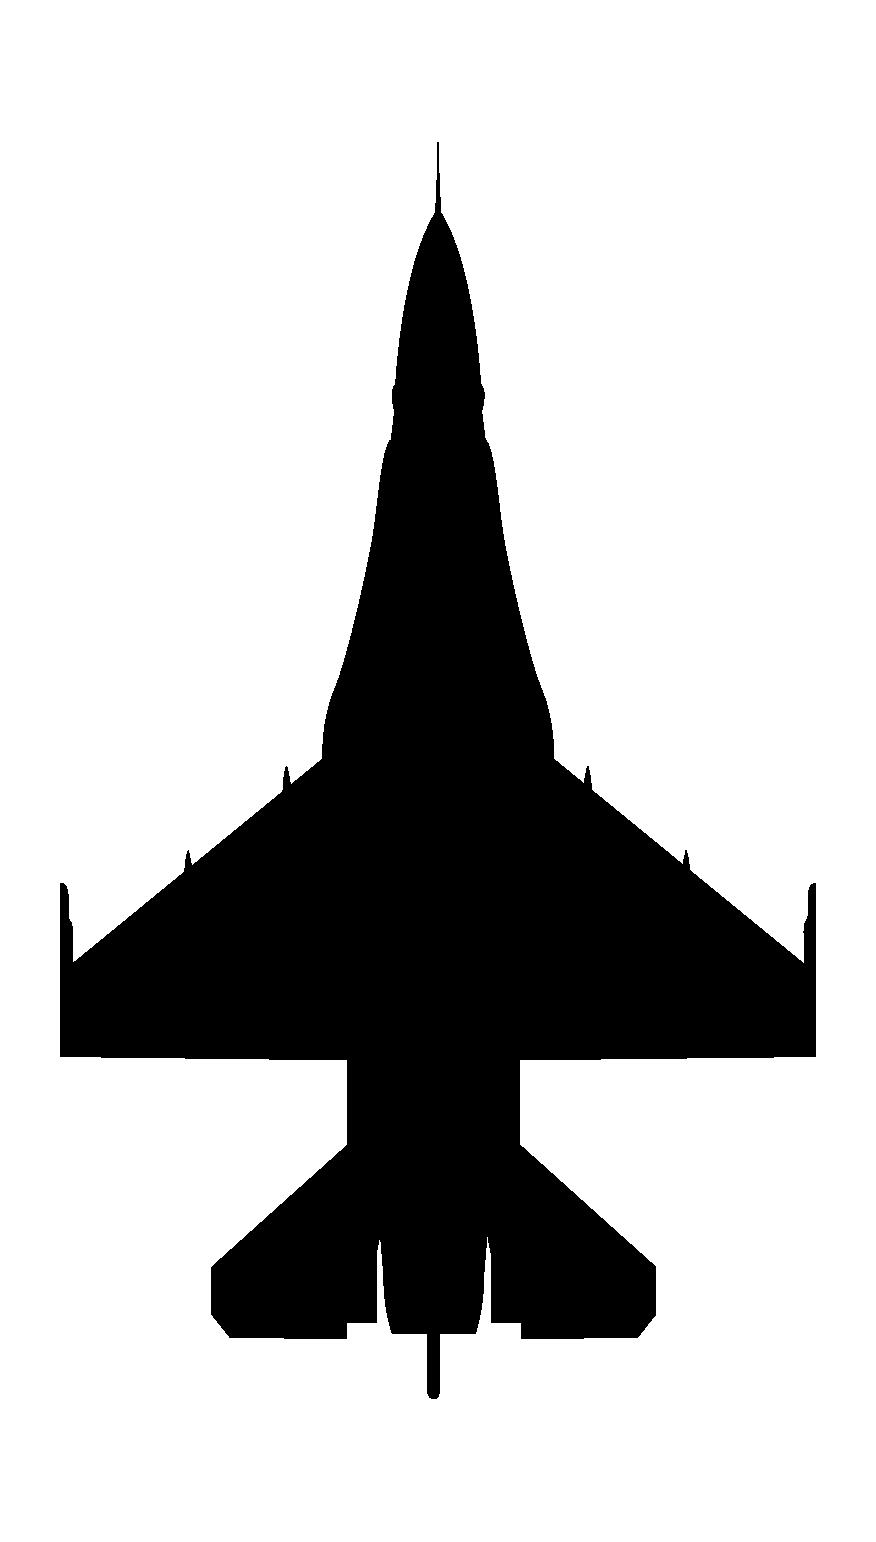
\includegraphics[
                        angle=0,
                        width=7.5mm,
                ]{diagrams/aircraft/silhouette_f16_top.pdf}};

            % bandit
            \node[] at (bandit) {
                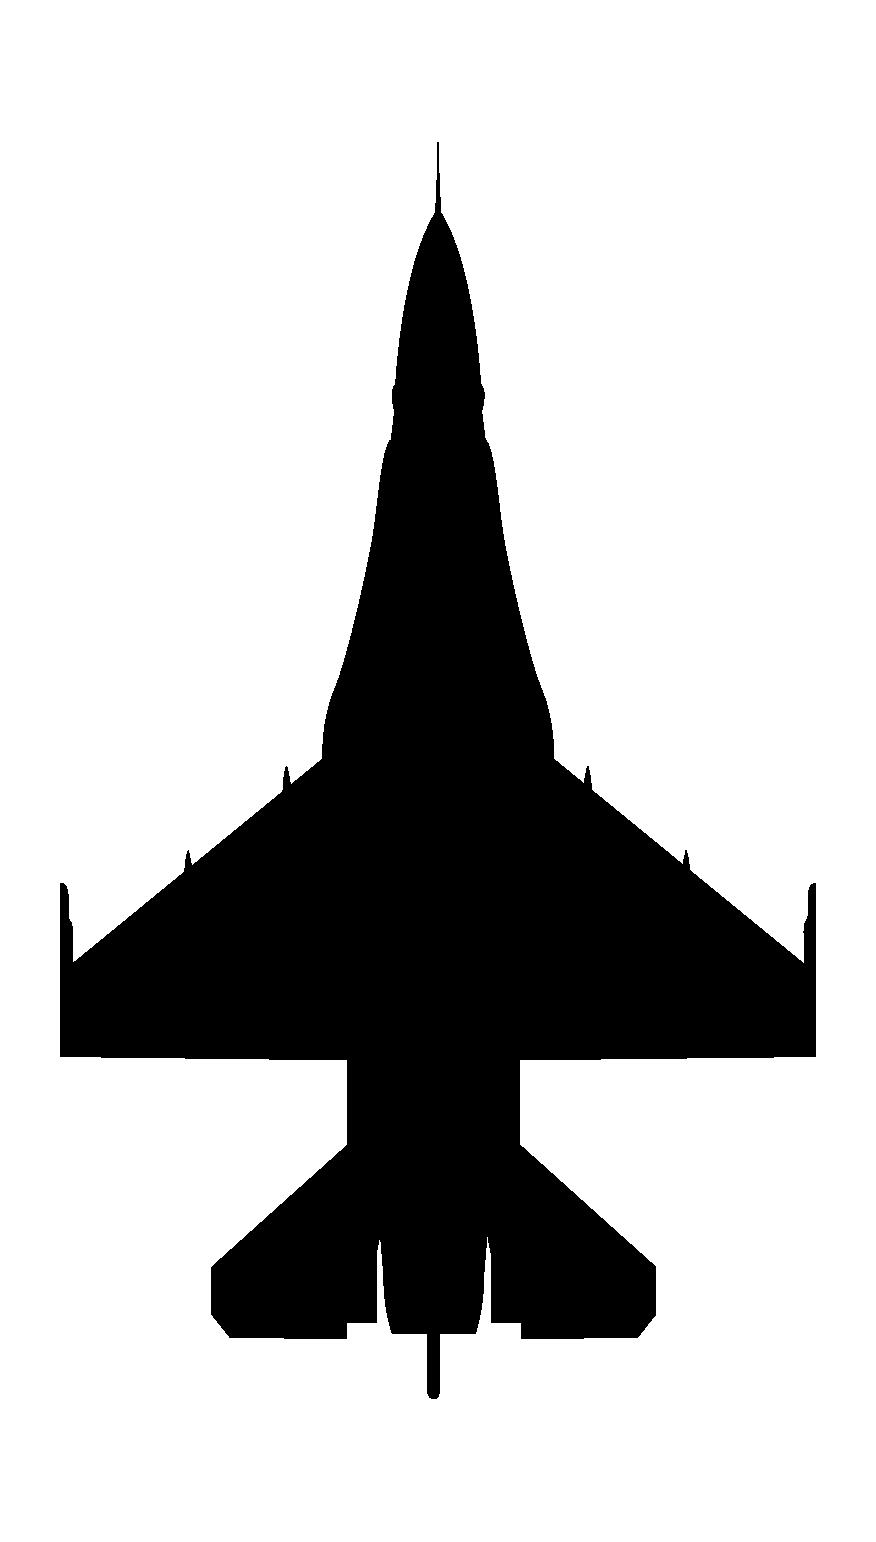
\includegraphics[
                    angle=180,
                    width=7.5mm,
            ]{diagrams/aircraft/silhouette_f16_top.pdf}};

            % labels
            \node[left, align=right, font=\small] at (cr) {
                \ref{subsec:ttpaa:timeline:banzai:commit}
            };
            \node[left, align=right, font=\small] at (mtr) {
                \ref{subsec:ttpaa:timeline:banzai:target}
            };
            \node[left, align=right, font=\small] at (sort) {
                \ref{subsec:ttpaa:timeline:banzai:sort}
            };
            \node[left, align=right, font=\small] at (shoot) {
                \ref{subsec:ttpaa:timeline:skate:shoot}
            };
            \node[left, align=right, font=\small] at (dr) {
                \ref{subsec:ttpaa:timeline:banzai:notch}
            };
            \node[left, align=right, font=\small] at (fighter_banzai) {
                \ref{subsec:ttpaa:timeline:banzai:banzai}
            };
            \node[left, align=right, font=\small] at (fighter_abort) {
                \ref{subsec:ttpaa:timeline:banzai:abort}
            };

        \end{tikzpicture}
        \caption{Banzai timeline}
        \label{fig:ttpaa:timeline:banzai}
    }%
    \textbf{--- start of intercept timeline}
    \begin{itemize}
        \item AWACS picture or own FCR contacts meet briefed commit criteria
        \item flight leaves assigned patrol area
        \item \textbf{No later than CR}
    \end{itemize}

    \blueitem[Target]
    \label{subsec:ttpaa:timeline:banzai:target}
    \begin{itemize}
        \item target call indicates responsibility to \\
        engage group in accordance with ROE
        \item flight members obtain radar contact
        \item \textbf{No later than MTR}
    \end{itemize}

    \blueitem[Sort]
    \label{subsec:ttpaa:timeline:banzai:sort}
    \begin{itemize}
        \item flight members sort contacts
        \item flight members obtain FCR lock on assigned contact
    \end{itemize}

    \blueitem[MRM Employment]
    \label{subsec:ttpaa:timeline:banzai:shoot}
    \begin{itemize} 
        \item verify clear avenue of fire
        \item \textbf{crank post launch to minimize closure}
        \item \textbf{such that missile active before fighter reaches DR}
    \end{itemize}
    
    \blueitem[Notch]
    \label{subsec:ttpaa:timeline:banzai:notch}
    \begin{itemize} 
        \item notch predetermined time (15s)
        \item \textbf{No later than DR}
    \end{itemize}
    \blueitem[Banzai / Abort]
    \begin{enumerate}[label=\textbf{\arabic{enumi}\alph*.}]
        \item \blue{Abort} (spiked) --- \textbf{5G slicing turn}%
        \label{subsec:ttpaa:timeline:banzai:abort}%
        \item \blue{Banzai} (naked) --- recommit and engage%
        \label{subsec:ttpaa:timeline:banzai:banzai}%
    \end{enumerate}
    
\end{checklistenumerate}

\clearpage

\subsection{SKATE TIMELINE}
\label{subsec:ttpaa:timeline:skate}

\begin{checklistenumerate}[start=0]
    \blueitem[Pre-commit] maintain SA
    
    \begin{itemize}
        \item \textbf{Comms} --- monitor AWACS
        \item \textbf{Sensors} --- sanitize airspace
    \end{itemize}

    \blueitem[Commit]%
    \label{subsec:ttpaa:timeline:skate:commit}
    \marginpar{
        \captionsetup{type=figure}
        \centering
        \begin{tikzpicture}[figstyle]

            % coordinates
            \coordinate (fighter_start) at (0,0);
            \coordinate (bandit) at (5,80);

            \coordinate (cr) at (0,0);
            \coordinate (mtr) at (0,10);
            \coordinate (sort) at (0,20);
            \coordinate (tr) at (0,30);
            \coordinate (dor) at (0,40);
            \coordinate (mrr) at (15,20);
            \coordinate (shoot2) at (5,50);
            \coordinate (mar) at (5,55);
            \coordinate (wez) at (0,65);
            \coordinate (fighter_end) at (20,50);

            % range lines
            \draw[thin]
                (25,0) -- (25,80);

            \path let \p1=(bandit) in 
            node[font=\footnotesize,anchor=west] at (25,\y1) {BANDIT};
            \path let \p1=(wez) in 
            node[font=\footnotesize,anchor=west] at (25,\y1) {WEZ};
            \path let \p1=(mar) in 
            node[font=\footnotesize,anchor=west] at (25,\y1) {MAR};
            \path let \p1=(dor) in 
            node[font=\footnotesize,anchor=west] at (25,\y1) {DOR};
            \path let \p1=(mrr) in 
            node[font=\footnotesize,anchor=west] at (25,\y1) {MRR};
            \path let \p1=(tr) in 
            node[font=\footnotesize,anchor=west] at (25,\y1) {TR};
            \path let \p1=(mtr) in 
            node[font=\footnotesize,anchor=west] at (25,\y1) {MTR};
            \path let \p1=(cr) in 
            node[font=\footnotesize,anchor=west] at (25,\y1) {CR};

            
            
            \draw[thin, dashed] let \p1=(wez) in  
                (25,\y1) -- ++(-30, 0);
            \draw[thin, dashed] let \p1=(mar) in  
                (25,\y1) -- ++(-20, 0);
            \draw[thin, dashed] let \p1=(dor) in  
                (25,\y1) -- ++(-25, 0);
            \draw[thin, dashed] let \p1=(tr) in  
                (25,\y1) -- ++(-25, 0);
            \draw[thin, dashed] let \p1=(mrr) in  
                (25,\y1) -- ++(-10, 0);
            \draw[thin, dashed] let \p1=(mtr) in  
                (25,\y1) -- ++(-25, 0);
            \draw[thin, dashed] let \p1=(cr) in  
                (25,\y1) -- ++(-25, 0);

            % bandit wez
            \draw[fill=red!40]
                (bandit)
                -- ++(-60:15)
                arc (-60:-120:15)
                -- (bandit);
            
            % timeline
            \draw[->] 
                (fighter_start) -- 
                node[below, pos=0]{
                    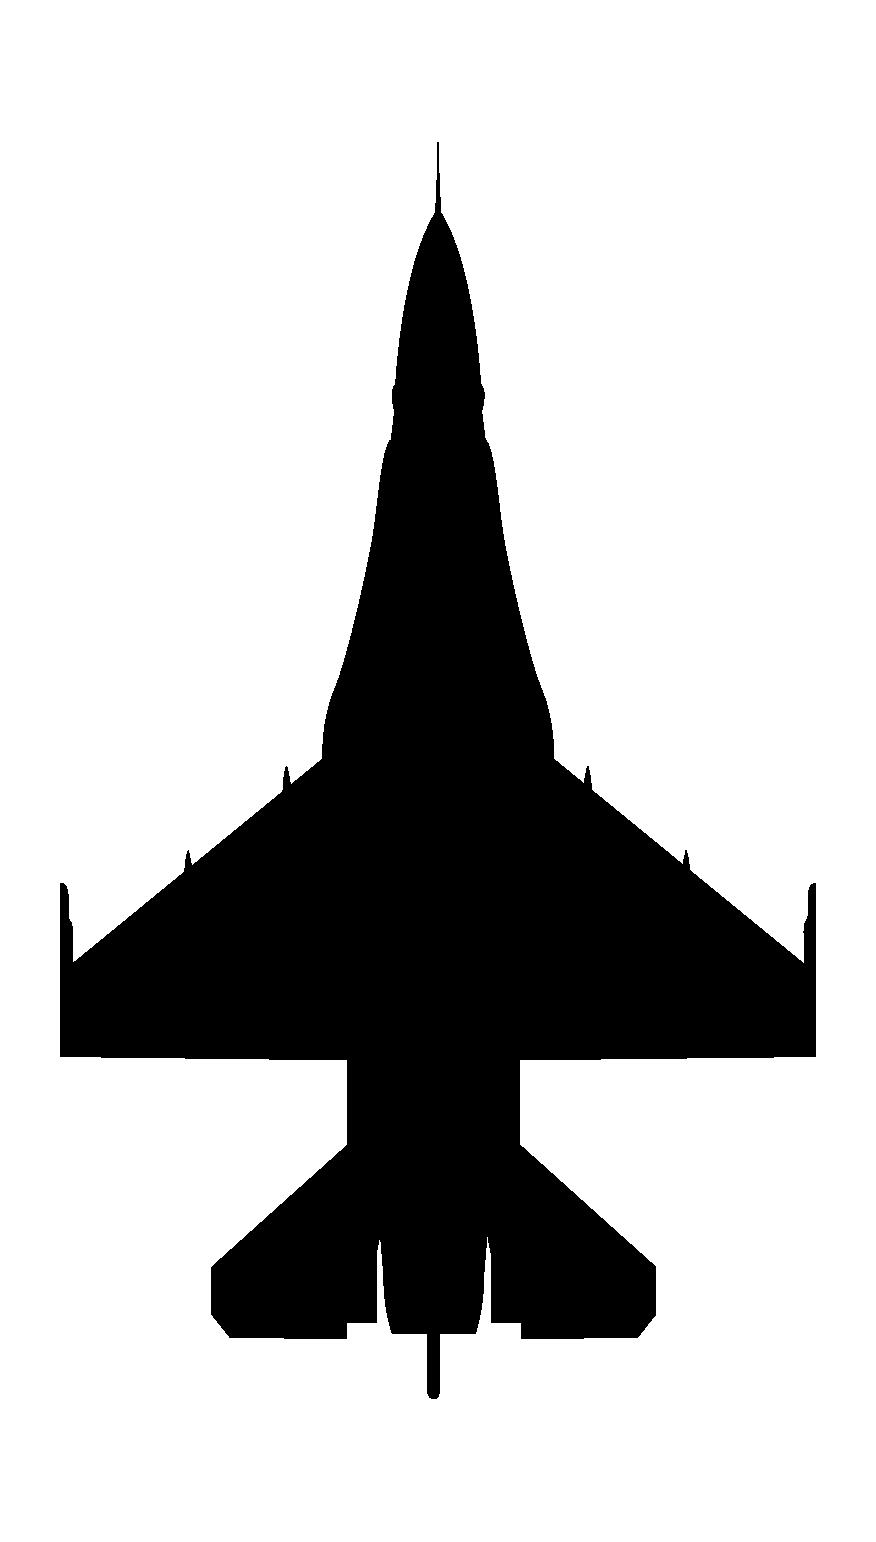
\includegraphics[
                    width=7.5mm,
                ]{diagrams/aircraft/silhouette_f16_top.pdf}} 
                (mtr);
            \draw[->]
                (mtr)
                -- (tr);
            \draw[->]
                (tr)
                -- (dor);
            \draw[->]
                (dor)
                arc (180:90:5) 
                -- ++(5,0)
                arc (90:0:5) 
                -- (mrr);
            \draw[->]
                (mrr)
                arc (0:-180:5) 
                -- (mar);
            \draw[->]
                (mar)
                arc (180:90:5) 
                -- ++(5,0)
                arc (90:0:5) 
                -- (fighter_end)
                node[below, pos=1, ]{
                    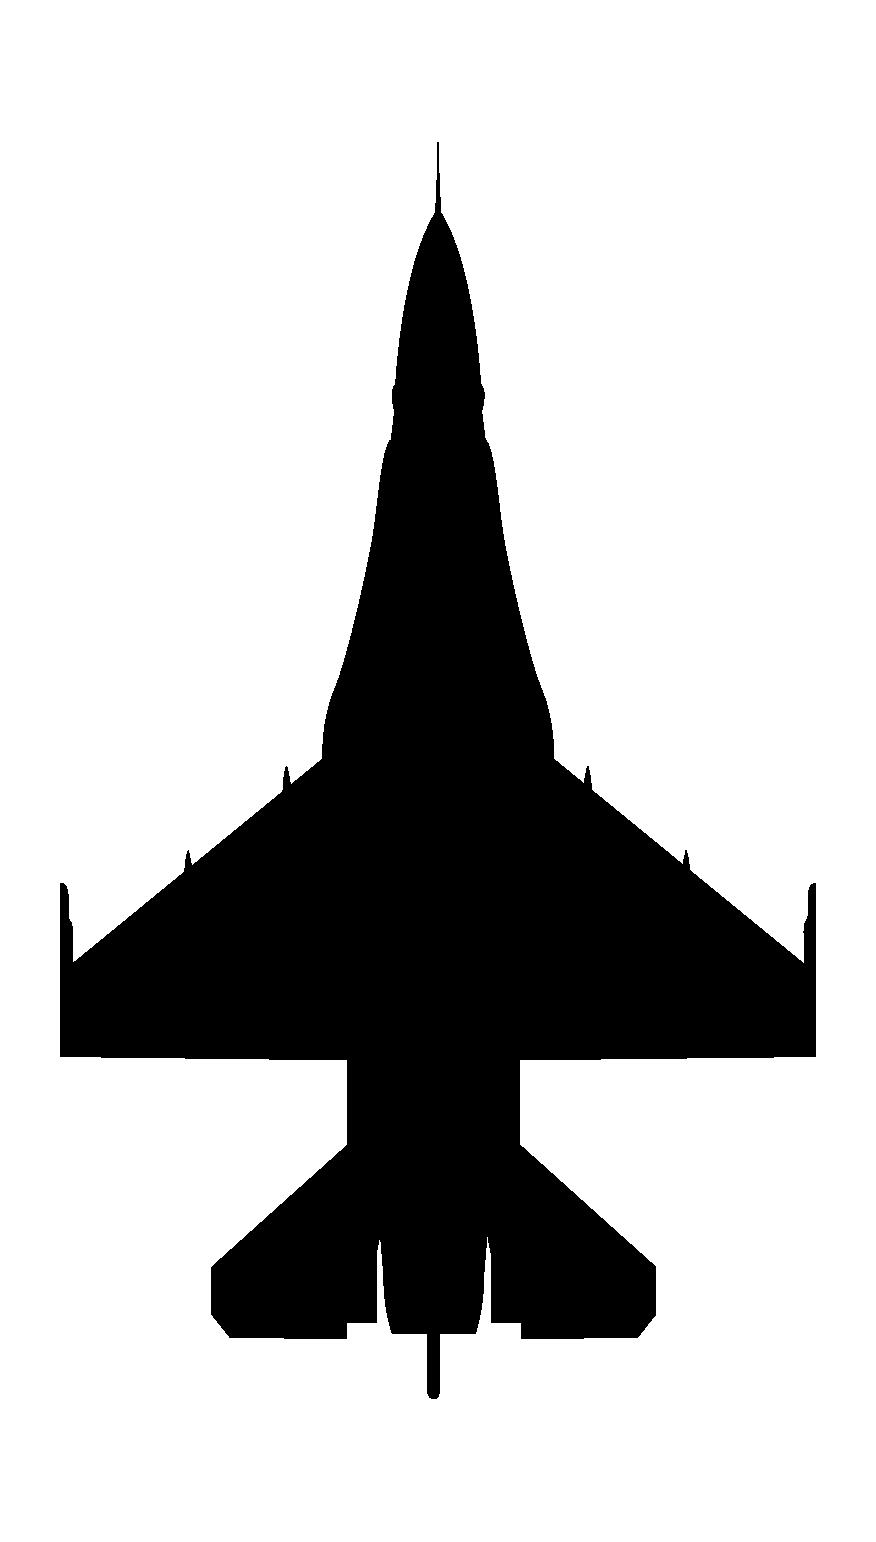
\includegraphics[
                        angle=180,
                        width=7.5mm,
                ]{diagrams/aircraft/silhouette_f16_top.pdf}};
            \draw[->, dashed]
                (mar)
                arc (180:90:5) 
                -- ++(5,0)
                arc (-90:0:5) 
                -- ++(0, 5)
                node[above, pos=1, ]{
                    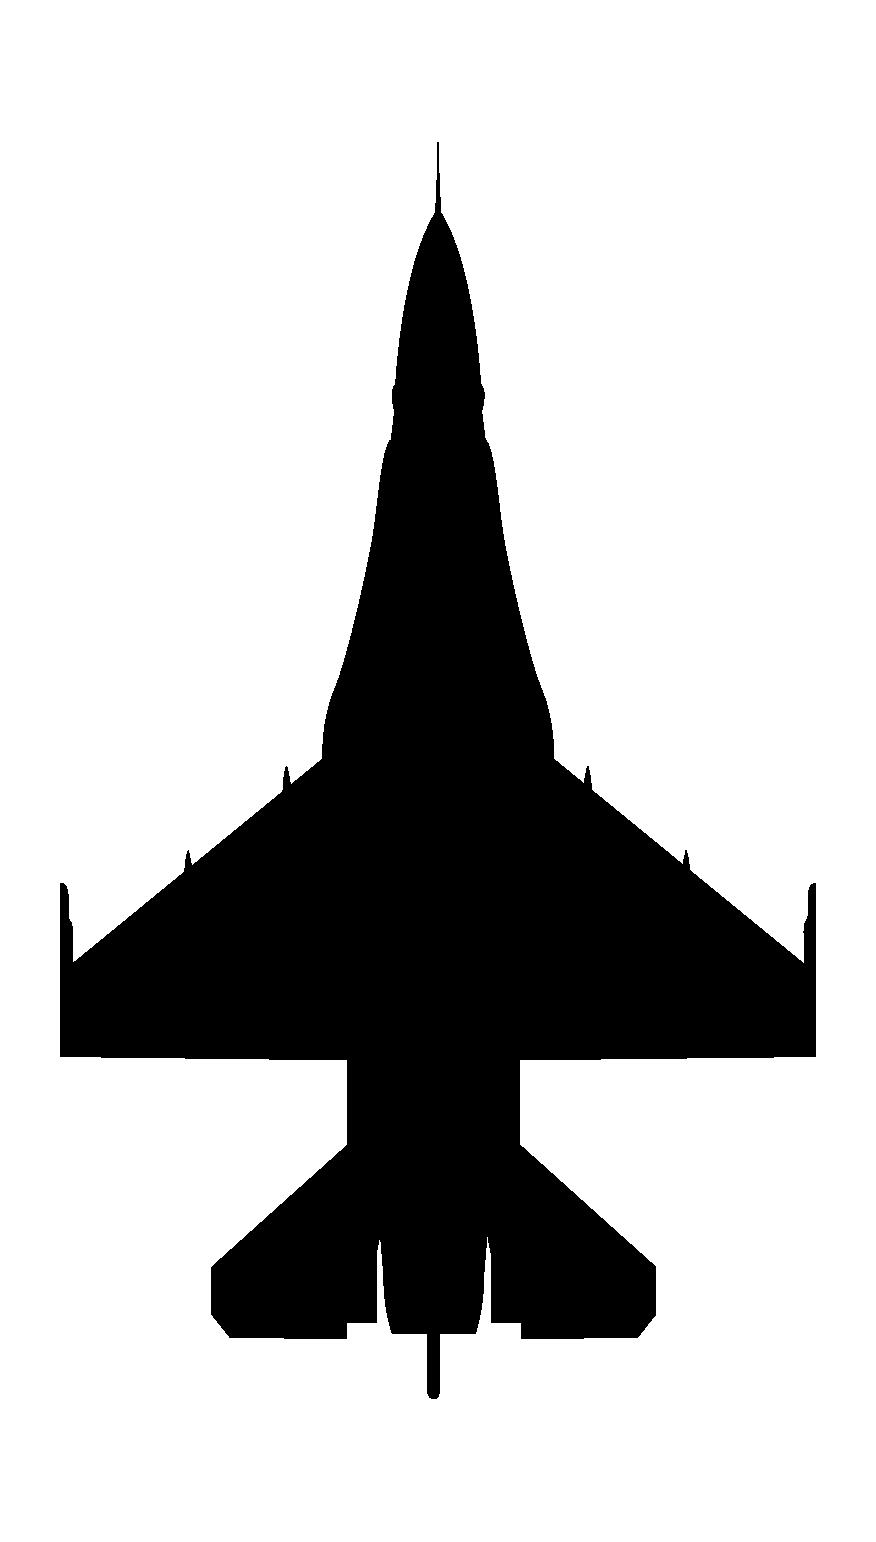
\includegraphics[
                        angle=0,
                        width=7.5mm,
                ]{diagrams/aircraft/silhouette_f16_top.pdf}};

            % bandit
            \node[] at (bandit) {
                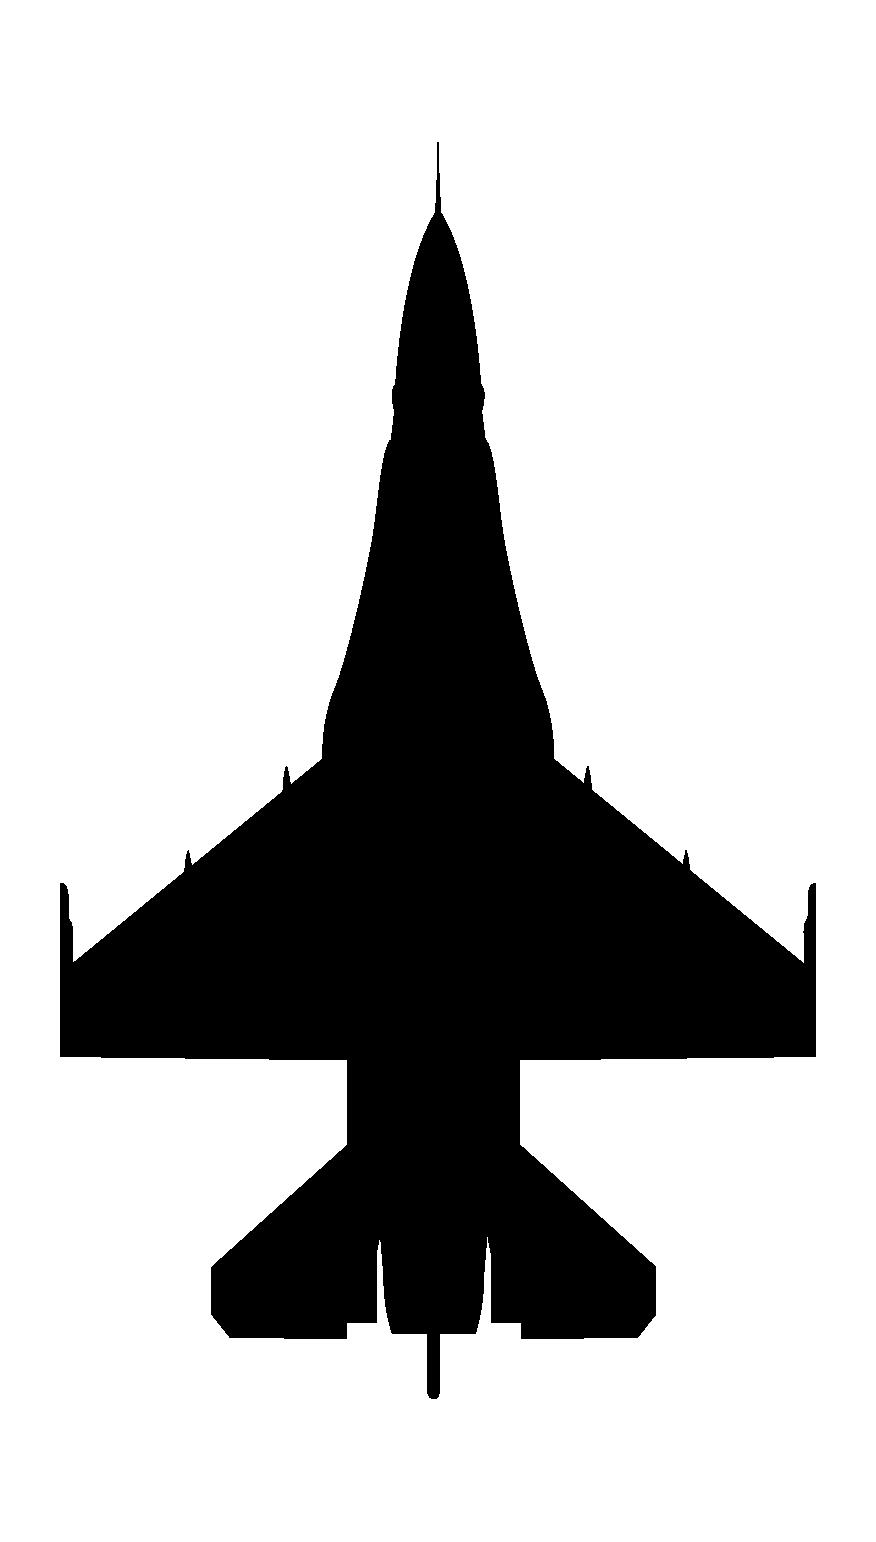
\includegraphics[
                    angle=180,
                    width=7.5mm,
            ]{diagrams/aircraft/silhouette_f16_top.pdf}};

            % labels
            \node[left, align=right, font=\small] at (cr) {
                \ref{subsec:ttpaa:timeline:skate:commit}
            };
            \node[left, align=right, font=\small] at (mtr) {
                \ref{subsec:ttpaa:timeline:skate:target}
            };
            \node[left, align=right, font=\small] at (sort) {
                \ref{subsec:ttpaa:timeline:skate:sort}
            };
            \node[left, align=right, font=\small] at (tr) {
                \ref{subsec:ttpaa:timeline:skate:shoot}
            };
            \node[left, align=right, font=\small] at (dor) {
                \ref{subsec:ttpaa:timeline:skate:out}
            };
            \node[left, align=right, font=\small] at (mrr) {
                \ref{subsec:ttpaa:timeline:skate:recommit}
            };
            \node[left, align=right, font=\small] at (shoot2) {
                \ref{subsec:ttpaa:timeline:skate:shoot2}
            };
            \node[left, align=right, font=\small] at (mar) {
                \ref{subsec:ttpaa:timeline:skate:abort}
            };

        \end{tikzpicture}
        \caption{Skate timeline}
        \label{fig:ttpaa:timeline:skate}
    }%
    \textbf{--- start of intercept timeline}
    \begin{itemize}
        \item AWACS picture or own FCR contacts meet briefed commit criteria
        \item flight leaves assigned patrol area
        \item \textbf{No later than CR}
    \end{itemize}

    \blueitem[Target]
    \label{subsec:ttpaa:timeline:skate:target}
    \begin{itemize}
        \item target call indicates responsibility to \\
        engage group in accordance with ROE
        \item flight members obtain radar contact
        \item \textbf{No later than MTR}
    \end{itemize}

    \blueitem[Sort]
    \label{subsec:ttpaa:timeline:skate:sort}
    \begin{itemize}
        \item flight members sort contacts
        \item flight members obtain FCR lock on assigned contact
    \end{itemize}

    \blueitem[MRM Employment]
    \label{subsec:ttpaa:timeline:skate:shoot}
    \begin{itemize} 
        \item verify clear avenue of fire
        \item \textbf{DLZ} --- R\textsubscript{PI} to R\textsubscript{OPT}
        \hfill (see \cref{fig:ttpaa:timeline:skate:dlz})\\
        manual loft to maximize performance
        \item \textbf{crank post launch to minimize closure}
        \item \textbf{No later than TR}
    \end{itemize}
    
    \marginpar{
        \captionsetup{type=figure}
        \centering
        \begin{tikzpicture}[figstyle]
            \node[boxedmarfigstyle] (fig) at (0,0) {
                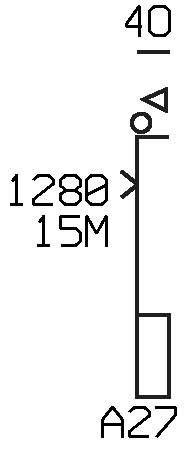
\includegraphics[
                    scale=0.5,
                ]{mfd/fcr_aa/aim120_subfig_dlz_prelaunch.pdf}
            };
        \end{tikzpicture}
        \caption{DLZ for skate}
        \label{fig:ttpaa:timeline:skate:dlz}
    }

    \blueitem[Out]
    \label{subsec:ttpaa:timeline:skate:out}
    \begin{itemize}
        \item \textbf{No later than DOR, after pitbull}
        \item 5G slicing turn
    \end{itemize}
    \blueitem[Recommit] (if necessary)
    \label{subsec:ttpaa:timeline:skate:recommit}
    \begin{itemize}
        \item \textbf{range must be greater than MRR}
        \item fighter must reacquire \& sort bandit
    \end{itemize}
    \blueitem[MRM Employment]
    \label{subsec:ttpaa:timeline:skate:shoot2}
    \begin{itemize}
        \item \textbf{No later than MAR}
    \end{itemize}
    \blueitem[Abort]%
    \label{subsec:ttpaa:timeline:skate:abort}
    \textbf{--- 5G slicing turn at MAR}
\end{checklistenumerate}

\clearpage

\subsection{SHORT SKATE TIMELINE}
\label{subsec:ttpaa:timeline:shortskate}

\begin{checklistenumerate}[start=0]
    \blueitem[Pre-commit] maintain SA
    
    \begin{itemize}
        \item \textbf{Comms} --- monitor AWACS
        \item \textbf{Sensors} --- sanitize airspace
    \end{itemize}

    \blueitem[Commit]%
    \label{subsec:ttpaa:timeline:shortskate:commit}
    \marginpar{
        \captionsetup{type=figure}
        \centering
        \begin{tikzpicture}[figstyle]

            % coordinates
            \coordinate (fighter_start) at (0,0);
            \coordinate (bandit) at (0,80);

            \coordinate (cr) at (0,0);
            \coordinate (mtr) at (0,10);
            \coordinate (sort) at (0,20);
            \coordinate (tr) at (0,30);
            \coordinate (msr) at (0,40);
            \coordinate (mar) at (0,55);
            \coordinate (wez) at (0,65);
            \coordinate (fighter_end) at (15,50);

            % range lines
            \draw[thin]
                (20,0) -- (20,80);

            \path let \p1=(bandit) in 
            node[font=\footnotesize,anchor=west] at (20,\y1) {BANDIT};
            \path let \p1=(wez) in 
            node[font=\footnotesize,anchor=west] at (20,\y1) {WEZ};
            \path let \p1=(mar) in 
            node[font=\footnotesize,anchor=west] at (20,\y1) {MAR};
            \path let \p1=(msr) in 
            node[font=\footnotesize,anchor=west] at (20,\y1) {MSR};
            \path let \p1=(tr) in 
            node[font=\footnotesize,anchor=west] at (20,\y1) {TR};
            \path let \p1=(mtr) in 
            node[font=\footnotesize,anchor=west] at (20,\y1) {MTR};
            \path let \p1=(cr) in 
            node[font=\footnotesize,anchor=west] at (20,\y1) {CR};

            
            
            \draw[thin, dashed] let \p1=(wez) in  
                (20,\y1) -- ++(-30, 0);
            \draw[thin, dashed] let \p1=(mar) in  
                (20,\y1) -- ++(-20, 0);
            \draw[thin, dashed] let \p1=(msr) in  
                (20,\y1) -- ++(-20, 0);
            \draw[thin, dashed] let \p1=(tr) in  
                (20,\y1) -- ++(-20, 0);
            \draw[thin, dashed] let \p1=(mtr) in  
                (20,\y1) -- ++(-20, 0);
            \draw[thin, dashed] let \p1=(cr) in  
                (20,\y1) -- ++(-20, 0);

            % bandit wez
            \draw[fill=red!40]
                (bandit)
                -- ++(-60:15)
                arc (-60:-120:15)
                -- (bandit);
            
            % timeline
            \draw[->] 
                (fighter_start) -- 
                node[below, pos=0]{
                    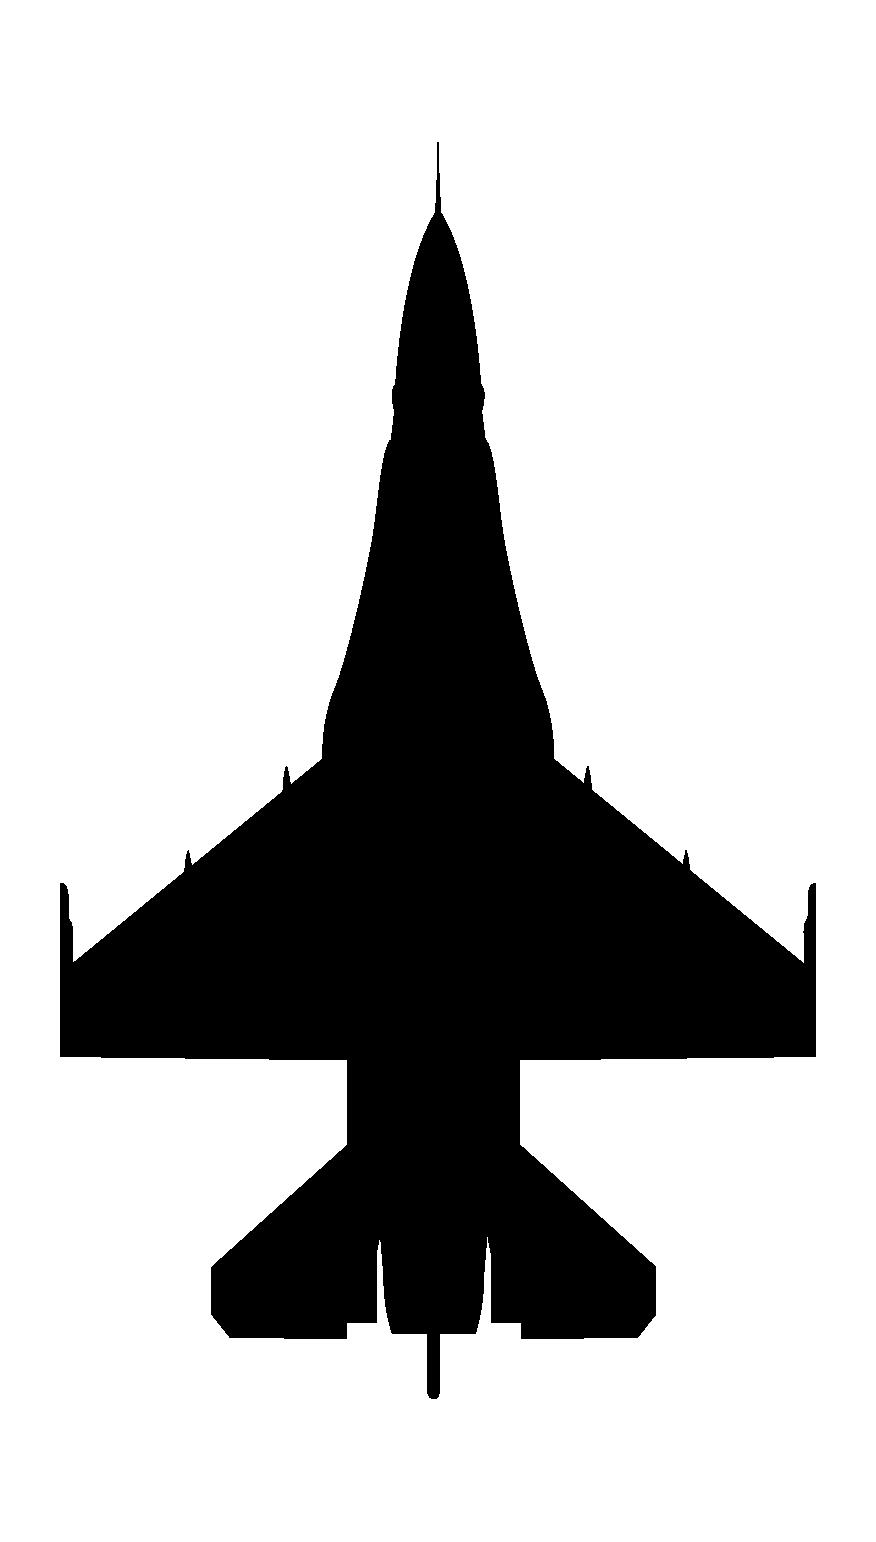
\includegraphics[
                    width=7.5mm,
                ]{diagrams/aircraft/silhouette_f16_top.pdf}} 
                (mtr);
            \draw[->]
                (mtr)
                -- (msr);
            \draw[->]
                (msr)
                -- (mar);
            \draw[->]
                (mar)
                arc (180:90:5) 
                -- ++(5,0)
                arc (90:0:5) 
                -- (fighter_end)
                node[below, pos=1, ]{
                    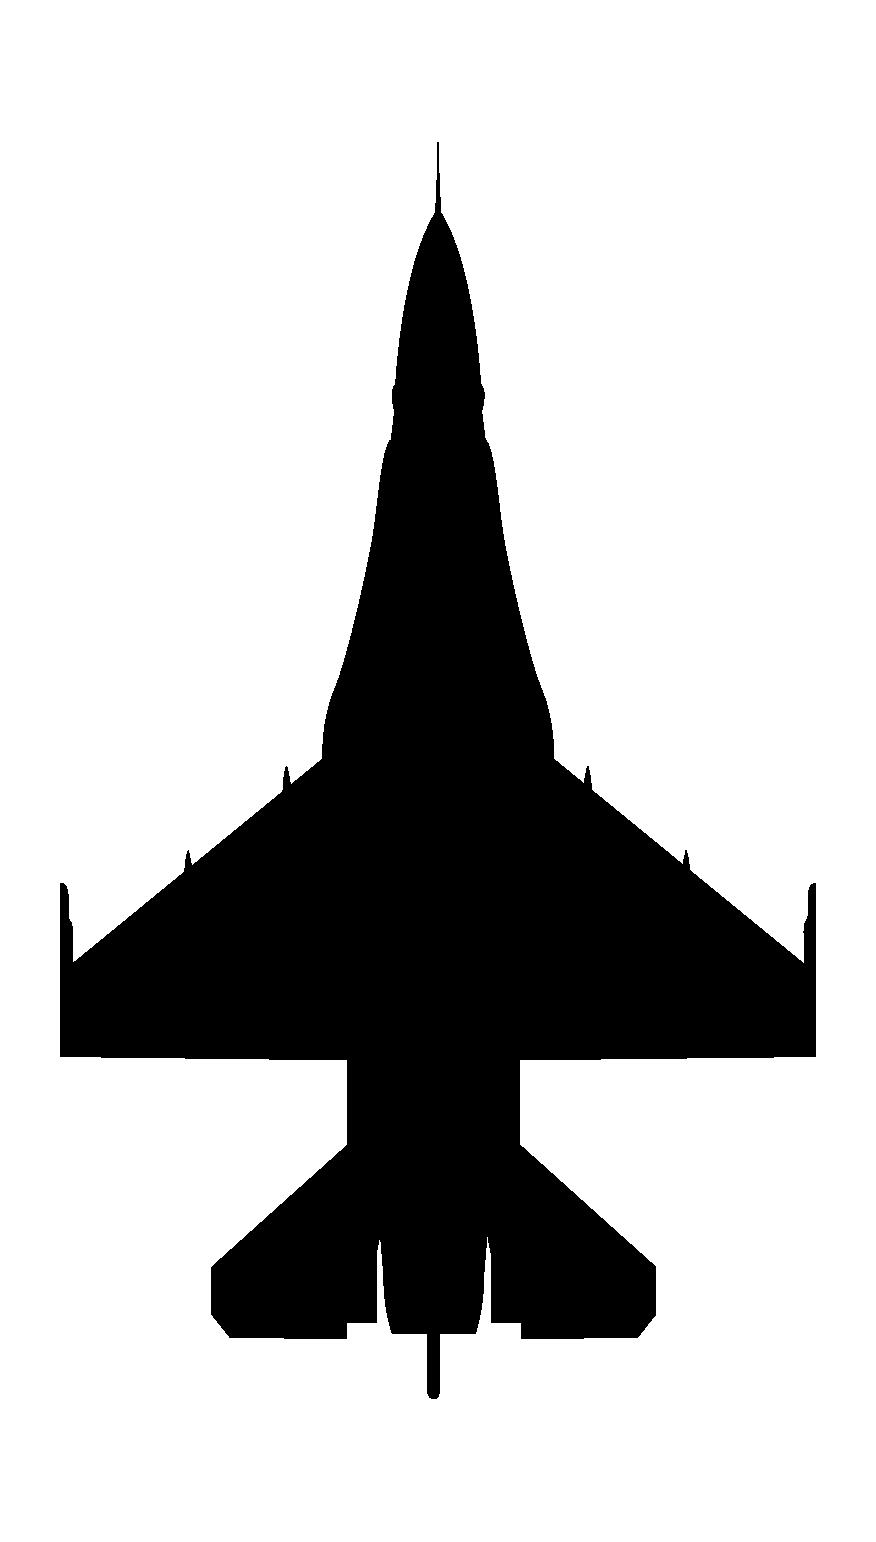
\includegraphics[
                        angle=180,
                        width=7.5mm,
                ]{diagrams/aircraft/silhouette_f16_top.pdf}};
            \draw[->, dashed]
                (mar)
                arc (180:90:5) 
                -- ++(5,0)
                arc (-90:0:5) 
                -- ++(0, 5)
                node[above, pos=1, ]{
                    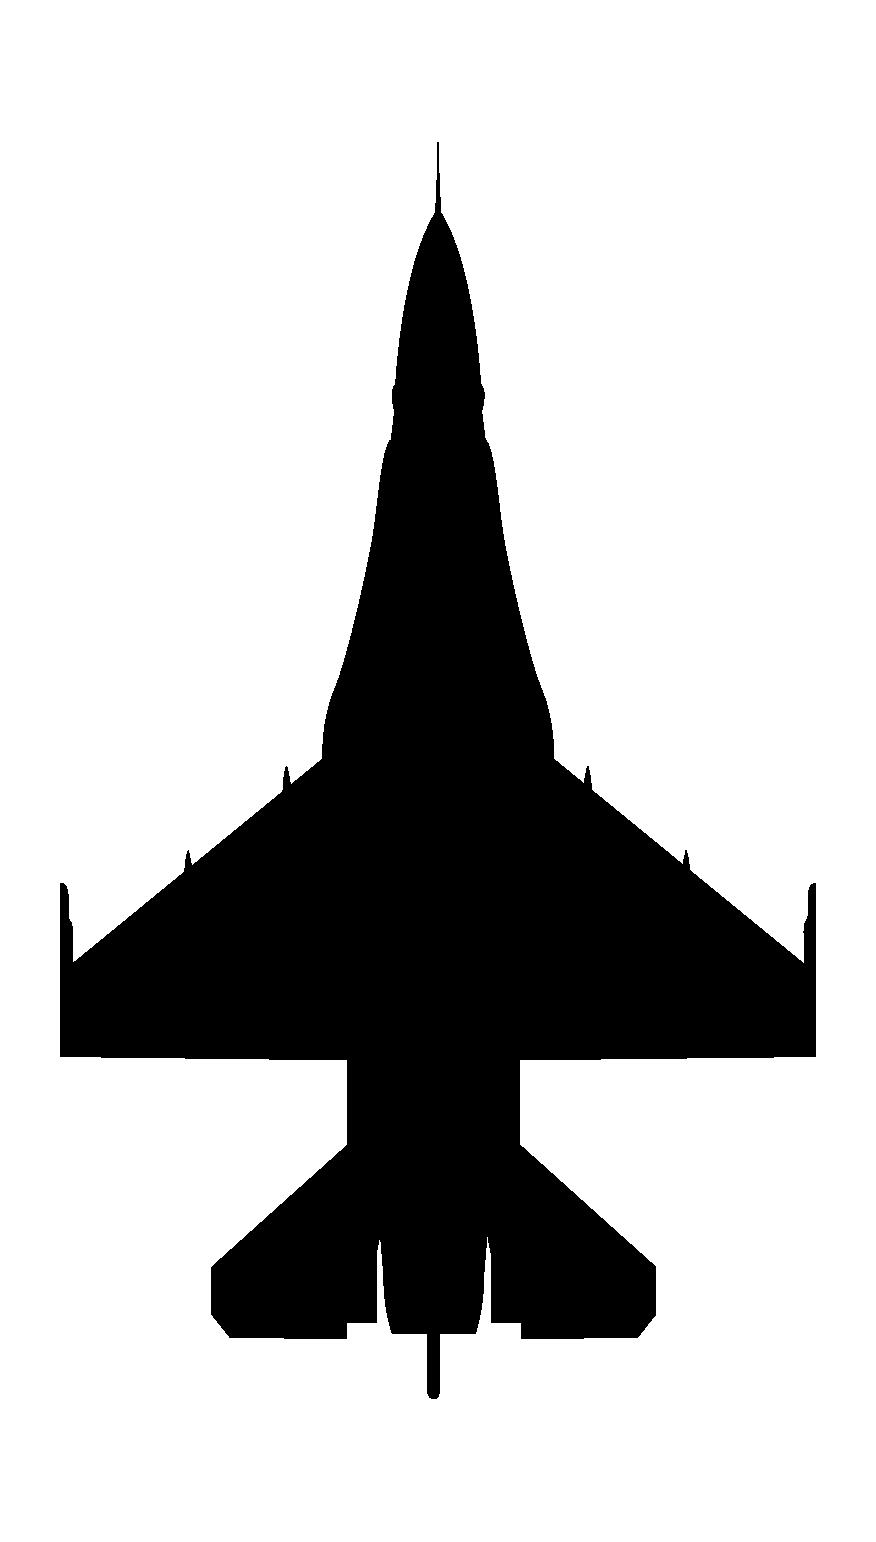
\includegraphics[
                        angle=0,
                        width=7.5mm,
                ]{diagrams/aircraft/silhouette_f16_top.pdf}};

            % bandit
            \node[] at (bandit) {
                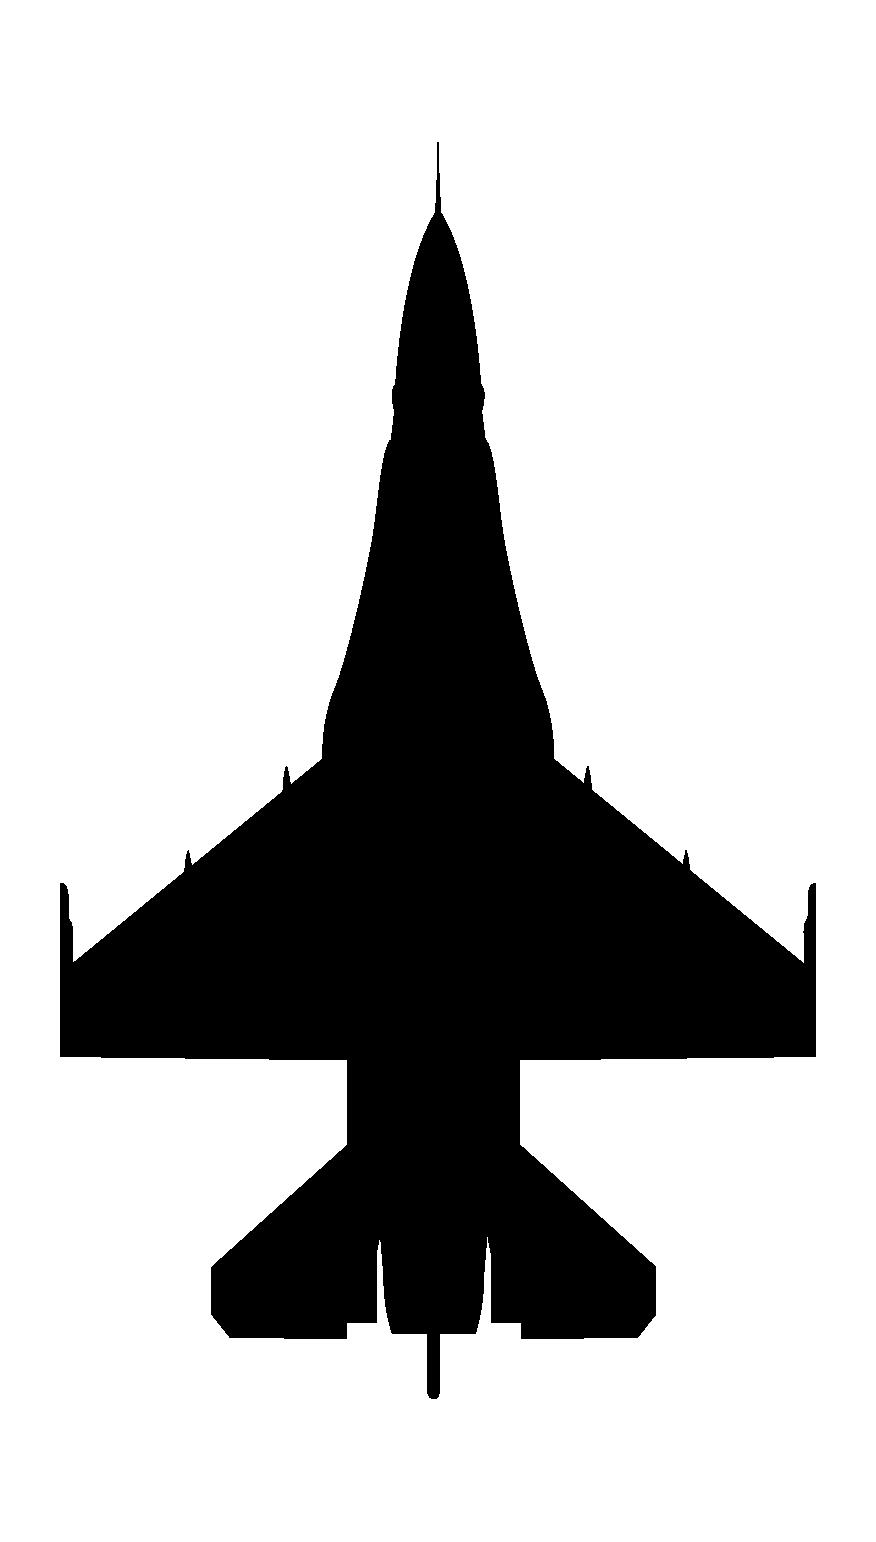
\includegraphics[
                    angle=180,
                    width=7.5mm,
            ]{diagrams/aircraft/silhouette_f16_top.pdf}};

            % labels
            \node[left, align=right, font=\small] at (cr) {
                \ref{subsec:ttpaa:timeline:shortskate:commit}
            };
            \node[left, align=right, font=\small] at (mtr) {
                \ref{subsec:ttpaa:timeline:shortskate:target}
            };
            \node[left, align=right, font=\small] at (sort) {
                \ref{subsec:ttpaa:timeline:shortskate:sort}
            };
            \node[left, align=right, font=\small] at (msr) {
                \ref{subsec:ttpaa:timeline:shortskate:shoot}
            };
            \node[left, align=right, font=\small] at (mar) {
                \ref{subsec:ttpaa:timeline:shortskate:abort}
            };

        \end{tikzpicture}
        \caption{Skate timeline}
        \label{fig:ttpaa:timeline:shortskate}
    }%
    \textbf{--- start of intercept timeline}
    \begin{itemize}
        \item AWACS picture or own FCR contacts meet briefed commit criteria
        \item flight leaves assigned patrol area
        \item \textbf{No later than CR}
    \end{itemize}

    \blueitem[Target]
    \label{subsec:ttpaa:timeline:shortskate:target}
    \begin{itemize}
        \item target call indicates responsibility to \\
        engage group in accordance with ROE
        \item flight members obtain radar contact
        \item \textbf{No later than MTR}
    \end{itemize}

    \blueitem[Sort]
    \label{subsec:ttpaa:timeline:shortskate:sort}
    \begin{itemize}
        \item flight members sort contacts
        \item flight members obtain FCR lock on assigned contact
    \end{itemize}

    \blueitem[MRM Employment]
    \label{subsec:ttpaa:timeline:shortskate:shoot}
    \begin{itemize} 
        \item verify clear avenue of fire
        \item \textbf{DLZ} --- R\textsubscript{TR} to R\textsubscript{PI} 
        \hfill (see \cref{fig:ttpaa:timeline:shortskate:dlz})\\
        manual loft to maximize performance
        \item \textbf{crank post launch to minimize closure}
        \item \textbf{within TR to increase P\textsubscript{K}}
        \item \textbf{No later than MSR}
        \item \textbf{no option to recommit and engage before MAR}
    \end{itemize}
    
    \marginpar{
        \captionsetup{type=figure}
        \centering
        \begin{tikzpicture}[figstyle]
            \node[boxedmarfigstyle] (fig) at (0,0) {
                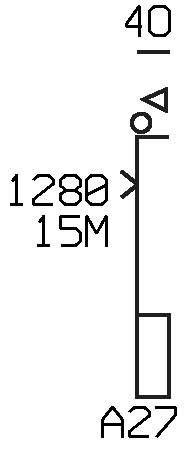
\includegraphics[
                    scale=0.5,
                ]{mfd/fcr_aa/aim120_subfig_dlz_prelaunch.pdf}
            };
        \end{tikzpicture}
        \caption{DLZ for short skate}
        \label{fig:ttpaa:timeline:shortskate:dlz}
    }
    \blueitem[Abort]%
    \label{subsec:ttpaa:timeline:shortskate:abort}
    \textbf{--- 5G slicing turn at MAR}
\end{checklistenumerate}

\marginfigrestore